%%!TEX encoding = UTF-8 Unicode

% Several lines in file have comments suggesting common packages for the
% typical thesis in informatics or electronics developed at UA
% uncomment/comment the lines as required for your work
% Before each optional line you will have a small comment

% According to UA rules, font size should range from 10 to 12pt.
\documentclass[11pt,a4paper,openright,twoside,onecolumn]{memoir}

\listfiles
\fixpdflayout

\usepackage[utf8]{inputenc}

% Select Computer Modern Typewritter (For bold ttfamily in listings)
\usepackage{lmodern}
% OR... Bera Mono
%\usepackage[scaled]{beramono} % TTT Font
%\usepackage{anyfontsize} % As the name says...


\usepackage[T1]{fontenc}

% Enable for for Overleaf support
\usepackage{ifthen}
\def\useoverleaf{0}  % change to non-zero (for instance, 1) to enable it

\makeatletter
\newcommand{\makecoverfile}[0]{%
  \immediate\write18{latexmk -pdf cover.tex}%
}
\makeatother


% For PDF merging
\usepackage{pdfpages}

% Set DPI to 300
\pdfpxdimen=\dimexpr 1in/300\relax

% Allow the use of a larger number of packages
\usepackage{morewrites} 

% For English and Portuguese languages
% Portuguese will be the default.
% Uncomment \setlanguage below to change it
\usepackage[english,portuguese]{babel}

% Uncomment to use a custom date format
%\usepackage{datetime}
%\newdateformat{thesisdate}{\monthname[\THEMONTH] \THEYEAR} % Month Year

% Make pdf look better
\usepackage{microtype} 

% Uncomment to enable floats on facing pages
%\usepackage{dpfloat}

% Side by side figures
% Eg. Fig 1a, Fig 1b
\usepackage[hang,small,bf]{caption}
%\let\tion\undefined
%\let\subfloat\undefined
\usepackage{subcaption}

%\RequirePackage{textcase}

% Dropped Caps
%\usepackage{lettrine}

% Configure Hyperlink color
% As a matter or style, you may use this to enable/disable color boxes on links
%\usepackage[breaklinks=true,colorlinks=false,linkcolor=blue]{hyperref}
% Or use the default values provided by the hyperref package
\usepackage{hyperref}

% Redefine section names according to your preference
%\def\sectionautorefname{Section}
%\def\chapterautorefname{Chapter}
%\def\figureautorefname{Figure}
%\def\listingautorefname{Listing}
%\def\tableautorefname{Table}

% Redefine code boxes
\ifthenelse{\equal{\useoverleaf}{0}}
{\usepackage[outputdir=build]{minted}}
{\usepackage{minted}}%

\addto\captionsportuguese{%
  \renewcommand\listingscaption{Código}
}
\fvset{fontsize=\footnotesize} % Make Code blocks smaller than text
\usepackage{csquotes}

% Add support for PDF Comments
\usepackage{comment}
\ifthenelse{\equal{\useoverleaf}{0}}
{\usepackage{pdfcomment}}{}
\usepackage{bookmark} % New Bookmarks

% For Multiple columns in Glossary
\usepackage{multicol}

% Add support for Math symbols
\usepackage{amsmath}
\usepackage{amssymb}

% Add support for graphics
\usepackage{graphicx}

% Add support for Colors
\usepackage{xcolor}

% Add support for the Euro symbol
\usepackage{eurosym}

% Add support for missingfigure and todo
\usepackage{todonotes}

% Setup bibliography with Biber using IEEE style for proper UTF-8 support
\usepackage[backend=biber, style=ieee, sorting=none, natbib=true, mincitenames=1, maxcitenames=2]{biblatex}
\bibliography{bib/references.bib, bib/rfc.bib}

% Use acronyms
\usepackage[printonlyused]{acronym} % For acronyms

% Indenting the first paragraph after section start
\usepackage{indentfirst}

% For fixing listoflistings with memoir
\usepackage{xparse}


% Uncomment the next lines to enable chart support through pgf and tikz
% This may require you to install further packages in your Tex system
%\usepackage[version=0.96]{pgf}
%\usepackage{tikz}

% UML support
%\usepackage{pgf-umlsd}

% Trees, Arrows, Mindmaps and other popular objects
%\usetikzlibrary{arrows,shadows,trees,shapes,decorations,automata,backgrounds,petri,mindmap} % for pgf-umlsd

% Package to master SI units
\usepackage[detect-weight=true, binary-units=true]{siunitx}
% For Electric Circuits
%\sisetup{load-configurations = binary}

% Set Voltage direction accordingly
% Option : oldvoltagedirection,nooldvoltagedirection,RPvoltages,EFvoltages
% More information at: https://mirrors.ibiblio.org/CTAN/graphics/pgf/contrib/circuitikz/doc/circuitikzmanual.pdf
% By default this template is using the Old Voltage Direction
%\usepackage[oldvoltagedirection,american,cuteinductors,smartlabels]{circuitikz}
%\usetikzlibrary{calc}
%\ctikzset{bipoles/thickness=1}
%\ctikzset{bipoles/length=0.8cm}
%\ctikzset{bipoles/diode/height=.375}
%\ctikzset{bipoles/diode/width=.3}
%\ctikzset{tripoles/thyristor/height=.8}
%\ctikzset{tripoles/thyristor/width=1}
%\ctikzset{bipoles/vsourceam/height/.initial=.7}
%\ctikzset{bipoles/vsourceam/width/.initial=.7}
%\tikzstyle{every node}=[font=\small]
%\tikzstyle{every path}=[line width=0.8pt,line cap=round,line join=round]

% For inline TT text (e.g. code snippets)
\usepackage{verbatim}

% Frames around figures and allow force placement
\usepackage{float}

% Configure Float style
%\floatstyle{boxed}
%\restylefloat{table}
%\restylefloat{figure}
%\restylefloat{lstlisting}

% For test purposes you may use the lipsum package to create dummy text
\usepackage{lipsum} % REMOVE

%Keep floats inside section!
\usepackage[section]{placeins}
\let \oldsubsubsection \subsubsection
\renewcommand{\subsubsection}[2][]{
  \FloatBarrier
  \oldsubsubsection#1{#2}
}
\let \oldsubsection \subsection
\renewcommand{\subsection}[2][]{
  \FloatBarrier
  \oldsubsection#1{#2}
}
\let \oldsection \section
\renewcommand{\section}[2][]{
  \FloatBarrier
  \oldsection#1{#2}
}
\let \oldchapter \chapter
\renewcommand{\chapter}[2][]{
  \FloatBarrier
  \oldchapter#1{#2}
}

% Glossary
\usepackage[%
    nogroupskip=false,%
    nonumberlist=true,%
    nopostdot=true,%
    % style=alttree,%
    style=listdotted,%
    % style=long,%
    % style=super,%
    shortcuts=abbreviations,%
    % The "uathesis" style file is already adding the glossary into the
    % table of contents.
    toc=false,%
]{glossaries-extra}


% Use the built-in division styling
\headstyles{memman}

% Include subsections in the TOC
\settocdepth{subsection}

% Numbering down to subsections as well
\setsecnumdepth{subsection}

% extra index for first lines
\makeindex[lines]

% Margins for University of Aveiro Thesis
\setlrmarginsandblock{3cm}{2.5cm}{*}
\setulmarginsandblock{3cm}{3cm}{*}
\checkandfixthelayout

% Or select your custom spacing to make any ajustment
%\addtolength{\parskip}{0.5\baselineskip}
\linespread{1.5}

\newcommand\mainmatterWithoutReset
{\edef\temppagenumber{\arabic{page}}%
  \mainmatter
  \setcounter{page}{\temppagenumber}%
}


%%%%%%%%%%%%%%%%%%%%%%%%%%%%%%%%%%%%%%%%%%%%%%%%%%
% Document begins here
%%%%%%%%%%%%%%%%%%%%%%%%%%%%%%%%%%%%%%%%%%%%%%%%%%

\begin{document}
\ifthenelse{\equal{\useoverleaf}{0}}{}{\makecoverfile{}}%
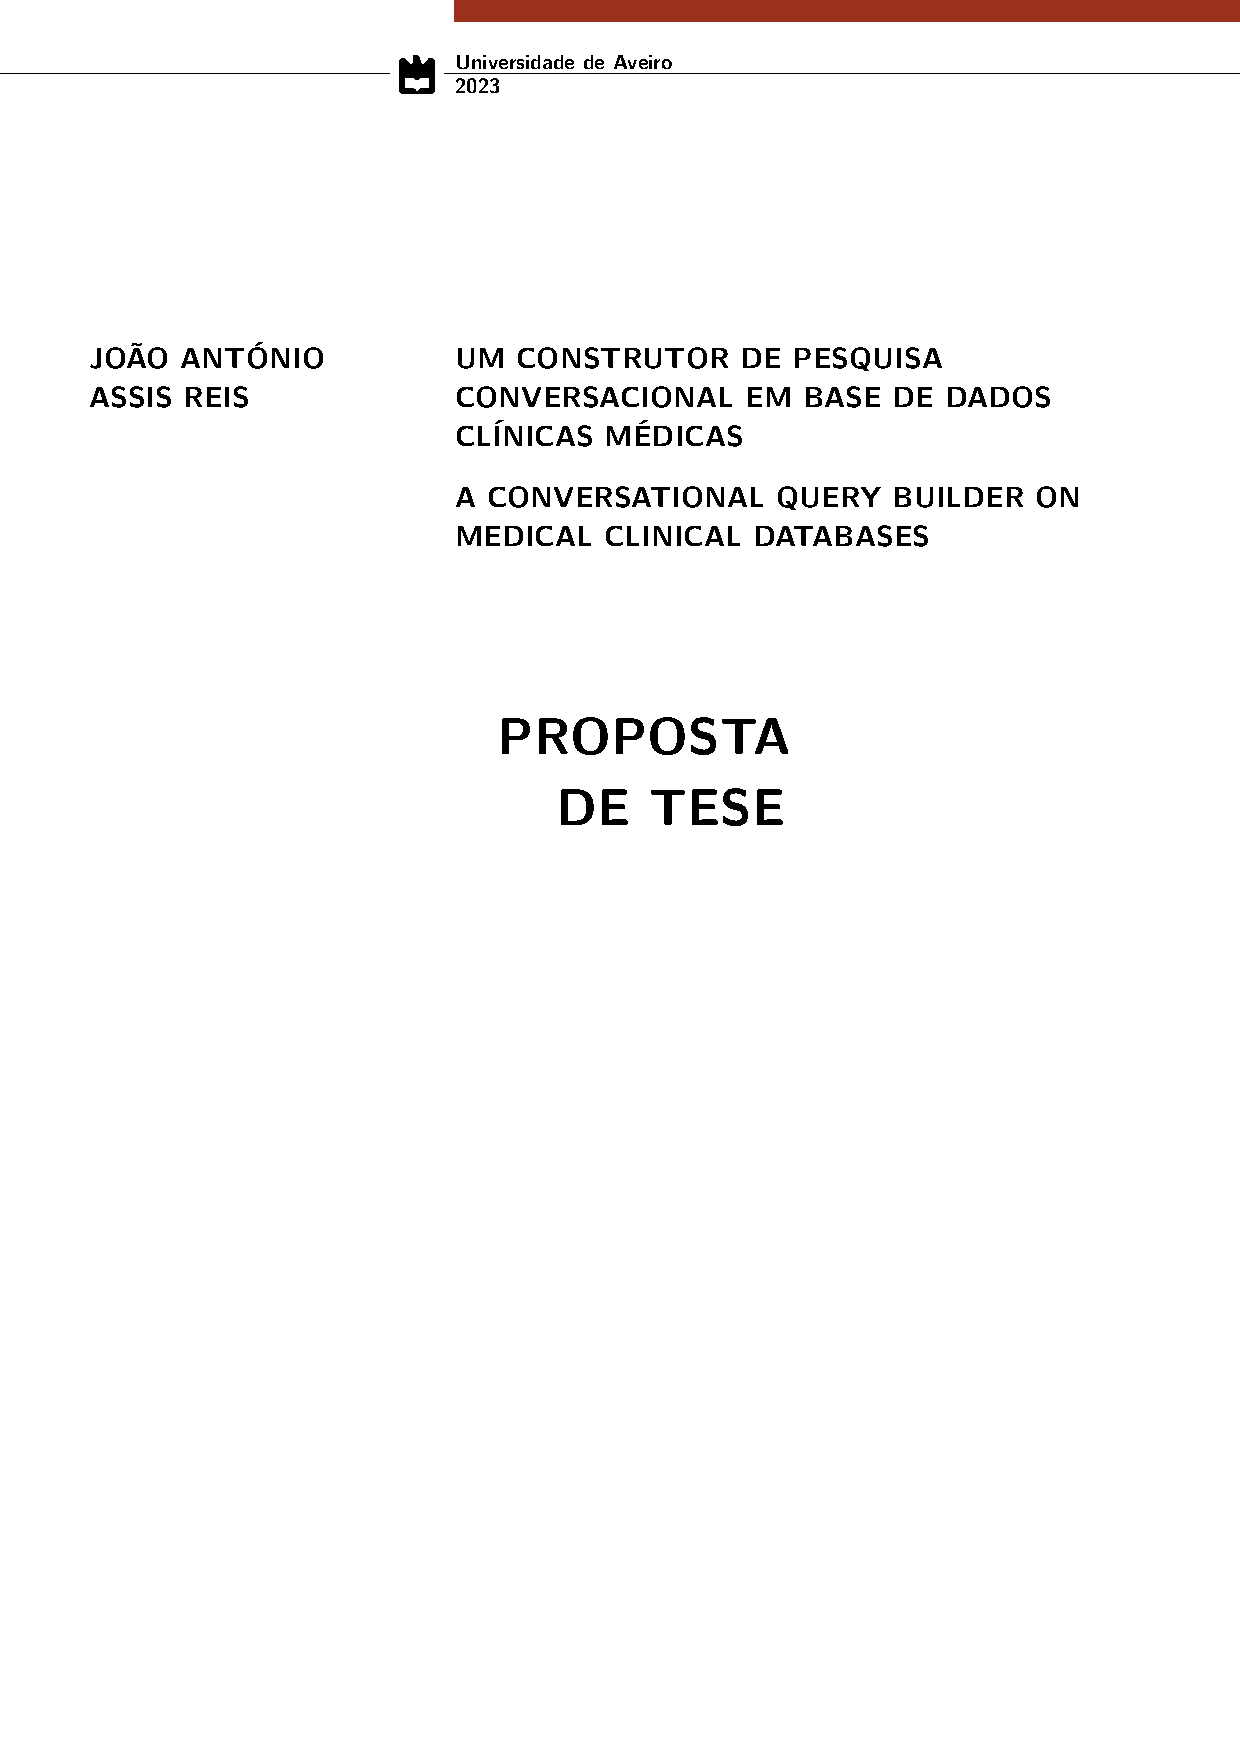
\includepdf[pages=-]{cover.pdf}

% Uncomment to enable English
\selectlanguage{english}


% Front matter

%Custom Chapter style named `thesis`
\makechapterstyle{thesis}{% Based on ell
  \chapterstyle{default}
  \renewcommand*{\chapnumfont}{\normalfont\sffamily}
  \renewcommand*{\chaptitlefont}{\normalfont\Huge\sffamily}
  \settowidth{\chapindent}{\chapnumfont 111}
  \renewcommand*{\chapterheadstart}{\begingroup
    \vspace*{\beforechapskip}%
    \begin{adjustwidth}{}{-\chapindent}%
    \hrulefill
    \smash{\rule{0.4pt}{15mm}}
    \end{adjustwidth}\endgroup}
  \renewcommand*{\printchaptername}{}
  \renewcommand*{\chapternamenum}{}
  \renewcommand*{\printchapternum}{%
    \begin{adjustwidth}{}{-\chapindent}
    \hfill
    \raisebox{10mm}[0pt][0pt]{\fontsize{30}{25}\selectfont\chapnumfont \thechapter}%
                              \hspace*{1em}
    \end{adjustwidth}\vspace*{-3.0\onelineskip}}
  \renewcommand*{\printchaptertitle}[1]{%
    \vskip\onelineskip
    \raggedleft {\chaptitlefont ##1}\par\nobreak\vskip 4\onelineskip}}


% Select chapter style from existing or select custom
%\chapterstyle{thesis} % Others: dowding, demo2, dash, chappell, brotherton, bianchi, ger, madsen, tatcher, veelo,indexes)
% thesis can also be used as defined previously
% Check the memoir documentation for the available themes
% Default is veelo
\chapterstyle{veelo}
\makeoddfoot{plain}{}{\thepage}{} % Added by André Zúquete to fix a page numbering issue on the veelo chapter style


% If you feel adventurous you can also define all aspects of your theme
% Use either this input or the chapterstyle before
% % Rules
\newcommand{\thinRule}{\rule{\textwidth}{0.25pt}}

% Customize heading appearances
% Define styles
\newcommand{\partSize}{\Huge}
\newcommand{\partStyle}{\lsstyle\scshape}
\newcommand{\chapterSize}{\Huge}
\newcommand{\chapterStyle}{\lsstyle\scshape}
\newcommand{\chapterAfter}{}
\newcommand{\sectionSize}{\Large}
\newcommand{\sectionStyle}{\scshape\MakeTextLowercase}
\newcommand{\subsectionSize}{\large}
\newcommand{\subsectionStyle}{\scshape\MakeTextLowercase}
\newcommand{\subsubsectionSize}{\large}
\newcommand{\subsubsectionStyle}{\scshape\MakeTextLowercase}
\newlength{\partNumSizePt}
\setlength{\partNumSizePt}{60pt}
\newlength{\chapterNumSizePt}
\setlength{\chapterNumSizePt}{60pt}
\newcommand{\partNumSize}{%
  \fontsize{\partNumSizePt}{1.2\partNumSizePt}\selectfont%
}
\newcommand{\partNumStyle}{\partChapterNumColor}
\newcommand{\chapterNumSize}{%
  \fontsize{\chapterNumSizePt}{1.2\chapterNumSizePt}\selectfont%
}
\newcommand{\chapterNumStyle}{\partChapterNumColor}

% Customize parts
\renewcommand{\partnamefont}{\partSize\partStyle}
\renewcommand{\partnumfont}{\partNumSize\partNumStyle}
\renewcommand{\printpartname}{}
\renewcommand{\printparttitle}[1]{%
  \normalfont\normalcolor\partnamefont #1
}

% Customize chapters
\makeatletter
\setlength{\beforechapskip}{30pt}
\renewcommand*{\chapterheadstart}{\vspace*{\beforechapskip}}
\setlength{\afterchapskip}{3ex}
\setlength{\midchapskip}{3ex}
\renewcommand*{\chapnamefont}{%
  \Large\flushright\chapterStyle\partChapterNumColor%
}
\renewcommand*{\chapnumfont}{\chapterNumSize\chapterNumStyle}
\renewcommand*{\chaptitlefont}{%
  \normalfont\flushleft\normalcolor\chapterSize\chapterStyle%
}
\renewcommand*{\printchaptername}{%
  \chapnamefont\MakeTextLowercase{\@chapapp}%
}
\renewcommand*{\chapternamenum}{\quad}
\renewcommand*{\printchapternum}{%
%  \chapnumfont\textls[-75]{\classicstylenums{\thechapter}}%
 \chapnumfont\textls[-75]{\thechapter}%

}
\renewcommand*{\printchaptertitle}[1]{%
  \chaptitlefont #1
  \chapterAfter
}
\makeatother
% Customize sections and subsections
\setsecnumformat{\csname my#1\endcsname\quad}
\setsecheadstyle{\sectionSize\sectionStyle}
\newcommand{\mysection}{{\thesection}}
\setlength{\beforesecskip}{3em}


\setsubsecheadstyle{\subsectionSize\subsectionStyle}
\newcommand{\mysubsection}{{\normalfont\subsectionSize\thesubsection}}
\setlength{\beforesubsecskip}{3em}

\setsubsubsecheadstyle{\subsubsectionSize\subsubsectionStyle}
\newcommand{\mysubsubsection}{{\normalfont\subsubsectionSize\thesubsubsection}}
\setlength{\beforesubsubsecskip}{2em}

% Customize "Table of ..." appearance
% Customize headings
\newcommand{\renewPrintXTitle}[1]{%
  \renewcommand{#1}[1]{%
    \printchaptertitle{##1}%
  }%
}
\renewPrintXTitle{\printtoctitle}
\renewPrintXTitle{\printlottitle}
\renewPrintXTitle{\printloftitle}

% Customize ToC headings
\renewcommand{\cftpartfont}{\partChapterNumColor\partStyle}
\renewcommand{\cftchapterfont}{\chapterStyle}
\renewcommand{\cftsectionfont}{}
\renewcommand{\cftsubsectionfont}{}
\renewcommand{\cftfigurefont}{}
\renewcommand{\cfttablefont}{}
\newcommand{\cftlstlistingfont}{}

% Increase number width
\newlength{\cftNumWidthIncrease}
\setlength{\cftNumWidthIncrease}{0.25em}
\addtolength{\cftpartnumwidth}{\cftNumWidthIncrease}
\addtolength{\cftchapternumwidth}{\cftNumWidthIncrease}
\addtolength{\cftsectionindent}{\cftNumWidthIncrease}
\addtolength{\cftsubsectionindent}{\cftNumWidthIncrease}
% No leader dots
%\renewcommand*{\cftpartdotsep}{\cftnodots}
%\renewcommand*{\cftchapterdotsep}{\cftnodots}
%\renewcommand*{\cftsectiondotsep}{\cftnodots}
%\renewcommand*{\cftsubsectiondotsep}{\cftnodots}
%\renewcommand*{\cftfiguredotsep}{\cftnodots}
%\renewcommand*{\cfttabledotsep}{\cftnodots}
%\newcommand*{\cftlstlistingdotsep}{\cftnodots}
% Set page numbers immediately after entry text
\newcommand{\tocEntryPageSep}{\hspace{1em}}
\renewcommand{\cftpartleader}{\cftdotfill{\cftdotsep}}
%\renewcommand{\cftpartafterpnum}{\cftparfillskip}
%\renewcommand{\cftchapterleader}{\tocEntryPageSep}
\renewcommand{\cftchapterleader}{\cftdotfill{\cftdotsep}}
%\renewcommand{\cftchapterafterpnum}{\cftparfillskip}
\renewcommand{\cftsectionleader}{\cftdotfill{\cftdotsep}}
%\renewcommand{\cftsectionafterpnum}{\cftparfillskip}
\renewcommand{\cftsubsectionleader}{\cftdotfill{\cftdotsep}}
%\renewcommand{\cftsubsectionafterpnum}{\cftparfillskip}
\renewcommand{\cftfigureleader}{\cftdotfill{\cftdotsep}}
%\renewcommand{\cftfigureafterpnum}{\cftparfillskip}
\renewcommand{\cfttableleader}{\cftdotfill{\cftdotsep}}
%\renewcommand{\cfttableafterpnum}{\cftparfillskip}
\newcommand{\cftlstlistingleader}{\cftdotfill{\cftdotsep}}
%\newcommand{\cftlstlistingafterpnum}{\cftparfillskip}
% Customize page numbers
\newcommand{\tocPageStyle}{\tocPageColor}
\renewcommand{\cftpartpagefont}{\tocPageStyle}
\renewcommand{\cftchapterpagefont}{\tocPageStyle}
\renewcommand{\cftsectionpagefont}{\tocPageStyle}
\renewcommand{\cftsubsectionpagefont}{\tocPageStyle}
\renewcommand{\cftfigurepagefont}{\tocPageStyle}
\renewcommand{\cfttablepagefont}{\tocPageStyle}
\newcommand{\cftlstlistingpagefont}{\tocPageStyle}

% Abstract
% Remove indents around abstract text
\setlength{\absleftindent}{0pt}
\setlength{\absrightindent}{0pt}
% Change font size to conform with the rest of the document text
\renewcommand{\abstracttextfont}{\normalsize}

% Customize headers and footers including page numbers
\newcommand{\hfTextSize}{\footnotesize}
\newcommand{\headTextStyle}{\lsstyle\scshape\MakeTextLowercase}
\nouppercaseheads
\makeevenhead{headings}%
             {\hfTextSize\thepage}%
             {}%
             {\hfTextSize\headTextStyle\leftmark}
\makeevenhead{plain}%
             {\hfTextSize\thepage}%
             {}%
             {\hfTextSize\headTextStyle\leftmark}
\makeoddhead{headings}%
            {\hfTextSize\headTextStyle\rightmark}%
            {}%
            {\hfTextSize\thepage}
\makeoddhead{plain}%
            {\hfTextSize\headTextStyle\rightmark}%
            {}%
            {\hfTextSize\thepage}


% Customize captions
\newcommand{\captionSize}{\small}
\newcommand{\captionStyle}{\scshape}
\newcommand{\captionWidthRatio}{0.9}

\captionnamefont{\captionSize\captionStyle}
\captiontitlefont{\captionSize}
\captiondelim{ -- }
\captiontitlefinal{}
\changecaptionwidth
%\captionwidth{\captionWidthRatio\textwidth}

% Define colors
%\newcommand{\titleColor}{\color[rgb]{0.616, 0.0627, 0.176}}
\newcommand{\titleColor}{\color[rgb]{0,0,0}}

\newcommand{\partChapterNumColor}{\titleColor}
\newcommand{\dropCapColor}{\titleColor}
%\newcommand{\tocPageColor}{\color[rgb]{0.0980, 0.329, 0.651}}

\newcommand{\tocPageColor}{\color[rgb]{0, 0,0}}
\definecolor{shade0}{rgb}{1.0 , 1.0 , 1.0 }
\definecolor{shade1}{rgb}{0.9 , 0.9 , 0.9 }
\definecolor{shade2}{rgb}{0.8 , 0.8 , 0.8 }
\definecolor{shade3}{rgb}{0.65, 0.65, 0.65}
\definecolor{shade4}{rgb}{0.45, 0.45, 0.45}
\definecolor{shade5}{rgb}{0.0 , 0.0 , 0.0 }



%Exclude sub figures from List of Figures
%\captionsetup[subfloat]{list=no}

% Texts
\newenvironment{introduction}
{%
  \begin{minipage}{\textwidth}%
   \itshape%
}
{%
  \end{minipage}%
  \par\addvspace{2\baselineskip plus 0.2\baselineskip minus 0.2\baselineskip}%
}

% Select Page style
\pagestyle{plain}


\frontmatter

\tightlists
\midsloppy
\raggedbottom

\setcounter{tocdepth}{2} %subsections are added to the TOC
\setcounter{secnumdepth}{4} %subsubsections are numbered

% Initial document tables start here: TOC, LOF, LOT, Glossary
% Table of contents with slightly smaller font
\cleardoublepage
{\small\tableofcontents}

% List of figures with slightly smaller font
\cleardoublepage
{\small\listoffigures}

% List of tables with slightly smaller font
\cleardoublepage
{\small\listoftables}

% List of code snippets

% Fix for Listings with memoir

\RenewDocumentCommand \chapter { s O{#3} m }{%
  \FloatBarrier
  \IfValueTF{#1}  % if optional star is seen
    {\oldchapter*{#2}}
    {\oldchapter#1{#2}}
}

\renewcommand{\listingscaption}{Código}
\renewcommand{\listoflistingscaption}{Lista de Excertos de Código}
\cleardoublepage
{\small\listoflistings}
\addcontentsline{toc}{chapter}{\listoflistingscaption}

% Reset Chapters
\renewcommand{\chapter}[2][]{
  \FloatBarrier
  \oldchapter#1{#2}
}

% Print Glossary
% {\small\chapter{Glossário}

\footnotesize
\SingleSpacing

\begin{multicols}{2}
\begin{acronym}[AAAAAA]

	\acro{ehden}[EHDEN]{European Health Data Evidence Network}
	\acro{omopcdm}[OMOP CDM]{Observational Medical Outcomes Partnership Common Data Model}
	\acro{ohdsi}[OHDSI]{Observational Health Data Sciences and Informatics}
	\acro{ir}[IR]{Information Retrieval}
	\acro{tf}[TF]{Term Frequency}
	\acro{idf}[IDF]{Inverse Document Frenquency}
	\acro{tfidf}[TF-IDF]{Term Frequency - Inverse Document Frenquency}
	\acro{dl}[DL]{Document Length}
	\acro{bm}[BM25]{Best Matching 25}
	\acro{qa}[QA]{Question Answering}
	\acro{ai}[AI]{Artificial Intelligence}
	\acro{nlp}[NLP]{Natural Language Processing}
	\acro{nlu}[NLU]{Natural Language Understanding}
	\acro{nlg}[NLG]{Natural Language Generation}
	\acro{lm}[LM]{Language Models}
	\acro{llm}[LLM]{Large Language Models}
	\acro{slm}[SLM]{Statistical Language Models}
	\acro{nlm}[NLM]{Neural Language Models}
	\acro{plm}[PLM]{Pre-trained Language Models}
	\acro{bert}[BERT]{Bidirectional Encoder Representations from Transformers}
	\acro{gpt}[GPT]{Generative Pre-trained Transformer}
	\acro{ml}[ML]{Machine Learning}
	\acro{rag}[RAG]{Retrieval-Augmented Generation}

\end{acronym}
\end{multicols}

}

% Print Glossary (glossaries-extra package)
\renewcommand{\glossaryname}{}
% {\printunsrtglossaries}



\newabbreviation
    {ir}
    {IR}
    {Information Retrieval}
\newcommand{\ir}{\gls{ir}}

\newabbreviation
    {tf}
    {TF}
    {Term Frequency}
\newcommand{\tf}{\gls{tf}}

\newabbreviation
    {idf}
    {IDF}
    {Inverse Document Frenquency}
\newcommand{\idf}{\gls{idf}}

\newabbreviation
    {tf-idf}
    {TF-IDF}
    {Term Frequency - Inverse Document Frenquency}
\newcommand{\tfidf}{\gls{tfidf}}

\newabbreviation
    {dl}
    {DL}
    {Document Length}
\newcommand{\dl}{\gls{dl}}


\newabbreviation
    {bm25}
    {BM25}
    {Best Matching 25}
\newcommand{\bm}{\gls{bm}}

\newabbreviation
    {qa}
    {QA}
    {Question Answering}
\newcommand{\qa}{\gls{qa}}

\newabbreviation
    {ai}
    {AI}
    {Artificial Intelligence}
\newcommand{\ai}{\gls{ai}}

\newabbreviation
    {nlp}
    {NLP}
    {Natural Language Processing}
\newcommand{\nlp}{\gls{nlp}}

\newabbreviation
    {nlu}
    {NLU}
    {Natural Language Understanding}
\newcommand{\nlu}{\gls{nlu}}

\newabbreviation
    {nlg}
    {NLG}
    {Natural Language Generation}
\newcommand{\nlg}{\gls{nlg}}

\newabbreviation
    {lm}
    {LM}
    {Language Models}
\newcommand{\lm}{\gls{lm}}

\newabbreviation
    {llm}
    {LLM}
    {Large Language Models}
\newcommand{\llm}{\gls{llm}}

\newabbreviation
    {slm}
    {SLM}
    {Statistical Language Models}
\newcommand{\slm}{\gls{slm}}

\newabbreviation
    {nlm}
    {NLM}
    {Neural Language Models}
\newcommand{\nlm}{\gls{nlm}}

\newabbreviation
    {plm}
    {PLM}
    {Pre-trained Language Models}
\newcommand{\plm}{\gls{plm}}

\newabbreviation
    {bert}
    {BERT}
    {Bidirectional Encoder Representations from Transformers}
\newcommand{\bert}{\gls{bert}}

\newabbreviation
    {gpt}
    {GPT}
    {Generative Pre-trained Transformer}
\newcommand{\gpt}{\gls{gpt}}

\newabbreviation
    {ml}
    {ML}
    {Machine Learning}
\newcommand{\mlearning}{\gls{mlearning}}


%%%%%%%%%%%%%%%%%%%%%%%%%%%%%%%%%%%%%%%%%%%%%%%%%%%%%%%
% Main document starts here
%%%%%%%%%%%%%%%%%%%%%%%%%%%%%%%%%%%%%%%%%%%%%%%%%%%%%%%

\mainmatter

% Line spacing: 1.5 pt 
\OnehalfSpacing

%%%%%%%%%%%%%%%%%%%%%%%%%%%%%%%%%%%%%%%%%%%%%%%%%%%%%%%
% Start of Thesis text 
%%%%%%%%%%%%%%%%%%%%%%%%%%%%%%%%%%%%%%%%%%%%%%%%%%%%%%%

% Uncomment to add further chapters
\chapter{Introduction}
\label{chapter:Introduction}

%\begin{introduction}
%
% 
%
%\end{introduction}

% falar sobre a historia de fazer estudos distribuidos...
% um investigador, várias BDs medicas, e existe um problema que as vezes ha falta de doentes numa BD. Surgiu a ideia de usarem multiplas DBs. Isto leva a outros problemas de iteroperabilidade. {\omop} e OHDSI.....

In the field of medical research, the lack of sufficient samples to conduct robust and statistically significant studies is still a challenge~\cite{rogers2021clinical}. This problem has more impact in studies involving rare diseases, specific patient subgroups, or when analyzing rare outcomes in common diseases~\cite{topaloglu2018using}. This lack of information can lead to underpowered studies, limiting the reliability and generalizability of the research findings~\cite{lombardo2023electronic}. Furthermore, the limitations imposed by insufficient data are significant since individual healthcare institutions often have limited patient populations, which restricts the diversity and volume of data available for research~\cite{rogers2021clinical,lombardo2023electronic}.

Multicentre studies are a possible strategy to overcome the issue of insufficient samples used in a study~\cite{almeida2021methodology}. By aggregating data from multiple sources, researchers may increase the number of participants and the population diversity~\cite{kaelber2008research}. Although this solution seems to solve the problem, it raises more challenges, namely the heterogeneity between databases~\cite{pereira2023querying} and privacy issues~\cite{almeida2022secure}. In other words, databases contain different types, formats, and/or sources, which are often not compatible with each other. The existence of these diverse data is not very effective, as they cannot be easily shared or integrated with other data.

To address the challenge of data heterogeneity in multi-institutional studies, the {\ohdsi} initiative proposed some strategies. {\ohdsi} is a collaborative network that aims to improve health by empowering a community to collaboratively generate evidence that promotes better health decisions and better care~\cite{hripcsak2016characterizing}. A key contribution of {\ohdsi} is the development of standardized data models and tools that facilitate the harmonization of observational health data~\cite{park2023exploring}. The most notable is the {\omop}. The {\omop} standardizes the format and content of clinical data, enabling data from different sources to be integrated and analyzed cohesively~\cite{hripcsak2016characterizing,almeida2021two}. The {\ohdsi} tools enable researchers to effectively overcome the barriers posed by data heterogeneity since the data would be mapped into the {\omop} format. This procedure also enhances the reproducibility and scalability of research, contributing to more reliable and impactful healthcare insights~\cite{reich2024ohdsi}.


\section{Motivation}
% 1º Problema: como econtrar as BDs? Alguem resolveu isso atraves de catalogues.... EHDEN
% 2º Problema: como é que eu escolho as bd de interesse nesses catalogues? Alguem criou uma forma de caracterizar essa BDs usando informações estatisticas e agregadas (Networkdashboards)
% 3º Problema: Ok isso é giro, mas algumas bd/conceitos são dispensos sendo dificil chegar à query que se pretende para o estudo. e este é o desafio


Solving the heterogeneity issues simplified the growth of multi-institutional observational databases. This raised new opportunities and challenges, considering multicentre studies~\cite{almeida2023clinical}. One of the main challenges is the selection of the most appropriate databases for conducting a study. However, there are already some solutions to address that problem~\cite{almeida2024montra2}. 

The {\ehden}project is one of several initiatives to simplify multicentre studies. In this project, the consortium members helped European data providers migrate their databases to the {\omop} data schema and publish their metadata in a web catalogue. This comprehensive catalogue offers researchers a centralized platform to explore the variety of available data sources~\cite{almeida2023fair}. With the increasing number of data partners, selecting databases only using metadata becomes complex, which leads to the creation of the {\ehden} Network Dashboards tool. It gives statistical and aggregated information about the databases available on the network. Researchers get more context to select, manually, the databases that satisfy their study requirements.

Despite these improvements, the catalogue now hosts the information of more than 150 databases. Researchers often spend considerable time and effort to find the most suitable database for their research criteria. The current methods of database discovery often rely on manual search and evaluation, which can be time-consuming and subject to human error, impacting the quality and efficiency of their research. For these reasons, the challenge of efficiently discovering the most appropriate databases for a specific study returned. 



\section{Objectives}

% How can a conversational query builder support medical researchers when defining a study protocol?
% Goals:
% 1. study of state-of-the-art
% 2. developed a chat-like search engine to help discover the best databases for a study
% 3. enhance the engine to collect additional information to provide a query as outcome.

With the increasing adoption of chatbot-like tools, the main objective of this work is to develop a conversational query builder to help medical researchers define their study objectives. This approach offers a more personalized and efficient method of database discovery. Researchers can interact with the chatbot conversationally, specifying their needs and receiving tailored recommendations. 

To achieve this objective, the present dissertation seeks to answer the following research question:

\begin{quote}
    \small\textit{How can a conversational query builder support medical researchers when defining a study protocol?}
\end{quote}

To answer this question, the work can be addressed by focusing on different aspects, namely by dividing it into three stages:

\begin{enumerate}
    \item Study of state-of-the-art: i) methodologies to build a conversational user interface, ii) procedures to retrieve the databases of most interest, and iii) explore the definition of a study protocol;
    \item Developed a chat-like search engine to help discover the best databases for a study;
    \item Enhance the engine to collect additional information to provide a query as an outcome. 
\end{enumerate}


\section{Dissertation outline}

% This dissertation follows the following structure: after an introduction, explaining the motivation, the problem and the proposed solution, follows the state of art where is described the current state of areas, tecnologies and techniques, such as Information Retrieval, Generative Artificial Inteligence and methods to define a study protocol.

This dissertation is organized into several sections, each designed to build upon the previous one to provide a comprehensive understanding of the project and its findings. The document starts with a introduction to provide background information, outlining the motivation, the problem and the proposed solution.

The introduction is followed by Chapter \ref{chapter:SA}, which delves into the state of the art. This chapter reviews the current literature and technologies relevant to the study. It aims to explore areas such as information retrieval procedures to access the most appropriate databases, large language models, methodologies to build a conversational user interface, interactive query builders, and the definition of a study protocol.

The Chapter \ref{chapter:CSA} and Chapter \ref{chapter:QB} describe the implementation phase. The Conversational Search Assistant, described in Chapter \ref{chapter:CSA}, aims to develop a chat-like search engine to help discover the best databases for a study. The Query Builder, outlined in Chapter \ref{chapter:QB}, explains how to enhance the engine to collect additional information to provide a query as an outcome.

This is followed by the Results and Discussion in Chapter \ref{chapter:RD}. It presents the findings of the study, analyzing and interpreting the results in the context of the research objectives.

To conclude the dissertation, the Chapter \ref{chapter:Conclusions} summarizes the findings and contributions of the project to this field.


\section{Contributions}

\noindent \textbf{Papers}

\begin{itemize}
    \item ``Using Flowise to Streamline Biomedical Data Discovery and Analysis''\cite{reis2024flowise}, 22nd IEEE Mediterranean Electrotechnical Conference (MELECON) 2024.
    \item ``A chatbot-like platform to enhance the discovery of OMOP CDM databases''\cite{MIE}, 34th Medical Informatics Europe (MIE) Conference 2024.
    \item ``HealthDBFinder: a question-answering task for health database discovery''\cite{CBMS}, 37th IEEE International Symposium on Computer-Based Medical Systems (CBMS) 2024.
\end{itemize}


\noindent \textbf{Posters}

\begin{itemize}
    \item OHDSI Collaborators Showcase Submission Form 2024.
\end{itemize}


\noindent \textbf{Presentations}

\begin{itemize}
    \item ``Using Flowise to Streamline Biomedical Data Discovery and Analysis''\cite{reis2024flowise} at 22nd IEEE Mediterranean Electrotechnical Conference (MELECON) 2024.
\end{itemize}
\chapter{State of Art}
\label{chapter: State of Art}

This dissertation suggests the development of a conversational query builder that functions as a chat-based interface within the EHDEN project ecosystem. This interface will help researchers redefine their studies effectively. The conversational virtual assistant will return a query to help discover the best databases for specific research. Studying state-of-the-art information retrieval systems to retrieve the most appropriate databases for a researcher's query is essential in this context. In addition, it is vital to explore the {\llm}, a recent advance of algorithms to perform {\nlp} tasks, and the actual state of conversational virtual assistants or chatbots. In the end, research about interactive query builder. And so these topics will be discussed below.


\section{Information Retrieval}

In computing and information science, {\ir} involves retrieving information from a database or multiple databases. According to \citet{p_m_efficient_2021}, the {\ir} system requires users to input queries, retrieving pertinent information from the database that aligns with the users' needs. Thus, this prevents the user from accessing a massive amount of information.

In conformity with \citet{hambarde_information_2023}, conventional text retrieval systems were predominant in the initial stages of the {\ir} field. These systems mainly depended on matching terms between queries and documents. Nevertheless, these systems based on terms have limitations, including issues like polysemy, synonymy, and linguistic gaps, which may restrict their effectiveness.

With the advancement of technology, deep learning techniques emerged, improving conventional text retrieval systems and overcoming the constraints associated with term-based retrieval methods. For this reason, the performance of these systems increased significantly, resulting in a more accurate and streamlined retrieval of information for end-users.

In turn, deep learning methods have evolved. Neural Network Architectures, transfer learning, and pre-training techniques emerged. These approaches have advanced the representation of textual data and bolstered the {\ir} system's comprehension of natural language queries.

More recently, Transformer architectures with attention mechanisms have been implemented in {\ir} systems to enable concentration on crucial query segments and documents for improved matching. Moreover, incorporating pre-trained language models like {\bert} and {\gpt}-2 has proven to enhance the performance of {\ir} systems, offering an advanced understanding of the semantics and context within natural language queries and documents.

This field has many applications in the real world. \citet{p_m_efficient_2021} highlights the following: streamlined and adaptable indexing and retrieval, information extraction, semantic matching, and multimedia retrieval. {\ir} generally functions across three main scales: searching the web, retrieving personal information, and conducting searches for enterprises, institutions, and domain-specific contexts.

In this section, I explored the {\ir} field, more specifically, how a {\ir} system works, what are the traditional methods and how {\ir} can be applied with {\nlp}.


\subsection{Overview of Information Retrieval Systems}

According to \citet{hambarde_information_2023}, an {\ir} system can be separated into two stages: Retrieval and Ranker. The following figure, adapted from \citet{hambarde_information_2023}, shows us an overview of modern {\ir} systems, highlighting the two main stages.

\begin{figure}[ht]
    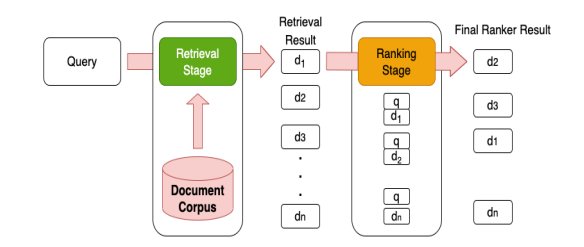
\includegraphics[width=14cm]{figs/chapter2/IR_system.png}
    \centering
    \caption{Overview of modern {\ir} system [REFAZER IMAGEM]}
\end{figure}

After analyzing the query, the retrieval stage will select an initial set of documents that are potentially pertinent to the query. Subsequently, the relevance of these documents undergoes reassessment through the similarity scores. The ranking is then refined using diverse algorithms and models, including the vector space model, Latent Semantic Indexing, Latent Dirichlet Allocation, and pre-trained models such as {\bert}.

This is followed by the ranking stage, in which the primary objective is to adjust the order of the initially retrieved documents based on their relevance scores. This phase prioritizes the enhancement of result effectiveness rather than efficiency. In the end, it returns a rank of documents as close as possible to the user's query criteria.


\subsection{Traditional Methods}

Some successful classical methods are {\tfidf} and {\bm}, briefly explained next.

\subsubsection{TF-IDF}

To understand the {\tfidf} method, first, it is necessary to understand the concepts of {\tf} and {\idf}. \citet{manning_introduction_2009} explained these concepts as follows.

It is reasonable to assume that a document containing a query term more frequently is more relevant to that query. Therefore, it should be assigned a higher relevance and/or score. So, {\tf} is the number of term occurrences in a document.

However, to evaluate the relevancy of a query, each term is regarded with equal importance, and this is the problem with the raw method explained above. \citet{manning_introduction_2009} clarified this with the following example: the automotive industry is expected to include the term "auto" in nearly every document. The  {\idf} calculates the rarity of a term across a set of documents. This measure is calculated as the logarithm of the inverse fraction of documents containing the term. The goal is to help prioritize some terms that are sporadic and possibly more informative.

The traditional {\ir} method, {\tfidf}, combines  {\tf} and  {\idf} definitions, as the name suggests, and then produces a weight for each term in each document, as \citet{manning_introduction_2009} and \citet{chizhik_challenges_2020} mention. The weight is calculated as the product of  {\tf} and  {\idf} values, highlighting terms that are both important within a specific document and relatively uncommon in the document collection. 

\begin{figure}[ht]
    
\includegraphics[width=6cm]{figs/chapter2/tf-idf_formula.png}
    \centering
    \caption{Overview of modern {\ir} system [REFAZER IMAGEM]}
\end{figure}

\citet{manning_introduction_2009} noted the {\tfidf} weight assigned to a term in a document is highest when the term frequently appears in a few documents, providing discriminating solid power. The weight is lower when the term occurs less frequently in a document or is widespread across many documents, indicating a less pronounced relevance signal. The weight is at its lowest when the term is present in nearly all documents. 

In summary, this {\ir} method evaluates the importance of a term within a document relative to its occurrence across a collection of documents.


\subsubsection{BM25}

{\bm}, the short form for Best Matching 25, is a ranking algorithm for {\ir} systems, especially in the context of search engines. It builds upon the {\tfidf} model to provide more accurate and context-aware document ranking. \citet{hambarde_information_2023} noted that {\bm} and other initial retrievers are employed for their effectiveness in recalling pertinent documents from an extensive pool.

The core components of {\bm} include {\tf}, {\idf}, {\dl}, and tuning parameters. Recapping from the {\tfidf} section, {\tf} is the number of occurrences that a specific term is in a document, and {\idf} is a measure that indicates the importance of a term in the whole document. 

\begin{figure}[ht]
    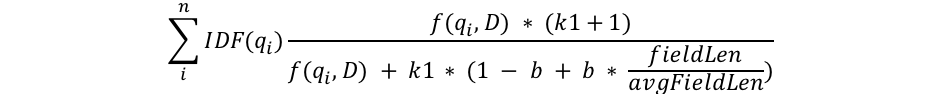
\includegraphics[width=14cm]{figs/chapter2/bm25_equation.png}
    \centering
    \caption{BM25 equation}
\end{figure}

As \citet{phd_understanding_2023} explained, the {\bm} equation is composed of the ith query term (q) and the respective {\idf} and {\tf} values. Also, include a division between the {\dl}, represented in the formula as fieldLen, and the average document length, avgFieldLen. This ratio evaluates how much the length of the document field deviates from the average length. So, the [https://www.elastic.co/blog/practical-bm25-part-2-the-bm25-algorithm-and-its-variables] explained intuitively: a document tends to receive a lower score when it contains more terms, especially those that do not match the query. The value b is a fine-tuning parameter, and it is responsible for length normalization. When b is larger, the ratio has a more significant effect on the overall score. Finally, the k1 value means term frequency saturation. It is a fine-tuning parameter that prevents the term frequency component of BM25 from having an unlimited impact on the document score.

This algorithm is simple and effective in {\ir} tasks, mainly search tasks. Also, it can handle vast collections. For these reasons, it is widely used and called a classic.

However, {\bm} can not perform a semantic analysis of the query and the documents, so getting the context and, in turn, getting better results is challenging. Another limitation is the ignorance of other crucial factors to get a better search beyond the factors relative to the {\tf} and {\dl}.


\subsection{IR in Question Answering}

{\qa} and {\ir} are closely related fields, together with {\nlp}. According to \citet{zhong_building_2020}, {\qa} aims to give users accurate and prompt responses to posed questions.

The traditional approach to question analysis and answering often involves mapping questions into predefined templates, such as "What-type" and "How-type". While widely utilized by existing online question-answering search engines, this template-based approach faces limitations in handling multiple questions. 

So, with the advancement of technology, another approach emerged: deep learning-based question-answering. In contrast with the traditional approach, this approach employs deep learning techniques, like convolutional neural networks (CNN), to offer automatic representation and analysis of questions. These neural models, trained through end-to-end approaches, excel in extracting and understanding complex characteristics in textual documents.

Recently, deep learning approaches with attention mechanisms and transfer learning have enhanced the flexibility of representation in text classification and named entity recognition. \citet{zhong_building_2020} highlights the tool {\bert}. {\bert} has emerged as a powerful model, utilizing contextualized representations for transfer learning. {\bert}-based models showcase performance in question-answering tasks, even in domains like medicine.



\subsubsection{Natural Language Processing (NLP)}

{\nlp} is the basis for building a {\qa} system. It is a field of {\ai} whose primary goal is to understand, interpret, and generate human language. The {\nlp} can be divided into two major components: {\nlu} and {\nlg}, according to \citet{ayanouz_smart_2020}

The \textbf{ {\nlu} } component plays a crucial role in processing and transforming unstructured data into a format the system can comprehend seamlessly. Essentially, the function of {\nlu} is to identify topics and entities, identify the intention, and determine the structure and syntax of the sentence.

In agreement with \citet{ngai_intelligent_2021}, for easy understanding by the chatbot, the user queries can be processed by semantic analysis, pragmatic analysis, and syntactic analysis. \citet{ayanouz_smart_2020} explained these steps and added two more necessary steps to make it easier to understand: a lexical analysis and discourse integration.

\begin{itemize}
    \item \textbf{Lexical Analysis}: This step involves analyzing and identifying the structure of words. It breaks down the text into chapters, sentences, phrases, and words. \citet{chizhik_challenges_2020} defined lexical analysis as the pre-processing of the text following the steps: tokenization, removal of special characters, links, and punctuation, and removal of stop-words.

    \item \textbf{Syntactic Analysis}: The syntactic analyzer parses the grammar and arrangement of words, making the relationships between different words more explicit. Essentially, it rejects sentences with incorrect structures. This analysis can be seen as the process of normalizing tokens.

    \item \textbf{Semantic Analysis}: This step ensures the text is meaningful and interprets its correct meaning by mapping syntactic constructions. It ensures that only semantically valid content is retained. The recognition of entities is part of this analysis.

    \item \textbf{Pragmatic Analysis and Discourse Integration}: This step analyzes the overall context to derive the conclusive interpretation of the actual message in the text. It considers factors like the true meaning of a phrase or sentence based on the broader context.
\end{itemize}

The other component is \textbf{{\nlg}}. Language generation is responsible for crafting coherent and linguistically accurate responses. Simply put, it grapples with the challenge of navigating the intricacies of natural human language. 



\section{Large Language Models}


It is crucial to trace briefly the development history to understand the concept of {\llm}. \citet{liu_prompting_nodate} explained this in a simple and intuitive way.

Before {\llm}, there were only simple {\lm}, which, in the initial stage, utilized a fully supervised learning approach, where task-specific models were trained on the target task dataset exclusively. Most of these were predictive models based on probabilities and Markov assumptions, also known as {\slm}. This was heavily dependent on feature engineering. Afterward, as deep learning gained prominence, an architecture designed to learn data features automatically; in other words, neural networks for {\nlp} emerged to enhance {\lm}’s capabilities. Integrating feature learning and model training, {\nlm} established a comprehensive neural network framework applicable to diverse {\nlp} tasks.

Most recently, in 2017, the launch of the self-attention mechanism revolutionized this field, and the Transformer architectures have become increasingly popular. These deep-learning architectures led to the development of pre-trained models not explicitly designed for a particular task, including {\bert} and {\gpt}, collectively known as {\plm}. {\plm} have shown significant performance enhancements across various {\nlp} tasks.

Following this, the researchers have involved the scale of model parameters, and the paradigm of “Pre-train, Prompt, Predict" like \citet{liu_prompting_nodate} call, gained widespread acceptance. So, in terms of interaction with {\lm}, the prompts became crucial. Researchers name these {\plm} with hundreds of billions of parameters as  {\llm}. Prompts effectively allow {\llm} to deal with a large number of complex and diverse tasks without a lot of effort.

In this section, I defined a {\llm}, explore briefily their architectures 


\subsection{Definition}

{\llm} are revolutionizing {\nlp} and {\ai} research. {\llm} are an {\ai} created to comprehend, generate, and engage in human language interactions. Essentially, these advanced {\ai} systems can mimic human intelligence. These models have a notable ability in natural language tasks, such as text generation and translation, {\qa}, decision-making, summarization, and sentiment analysis.

These models can process and predict patterns with great accuracy due to their significant model parameters, often comprising hundreds of billions of parameters. \citet{hadi_LLM_2023} combine sophisticated {\slm} and deep learning techniques to train, analyze, and understand huge volumes of data, learning the patterns and relationships among the data. For this reason, according to \citet{naveed_comprehensive_2023}, when provided with task descriptions and examples through prompts, {\llm} can produce textual responses to task queries. So, we can put {\llm} in the generative {\ai} field.

\citet{liu_prompting_nodate} say that the release of ChatGPT 1 garnered significant social attention, and research into {\llm} has evolved. This has led to the development of noteworthy products like PaLM, {\gpt}-2, {\gpt}-3, and, most recently, {\gpt}-4, and LLaMA and LLaMa-2.


\subsection{Architecture Overview}

\subsubsection{Transformer Architecture}

The development and advancement of {\llm} is thankful for the introduction of Transformers by \citet{vaswani_attention_2023} in 2017. Most {\llm} are built on the Transformer model, which is based on a self-attention mechanism and encoder-decoder structures. This new technology enables parallelization and efficient handling of long-range dependencies, according to \citet{hadi_LLM_2023}, and led to the development of models that have achieved enormous results, such as {\gpt} by OpenAI and {\bert} by Google.

The innovation of this model is due to the self-attention mechanism, one of the key components. It allows the model to weigh the importance of different words in a sequence when processing each word. This mechanism enables the model to focus on relevant information, capturing dependencies regardless of word order.

Another key component is the Encoder and Decoder Stacks. Essentially, the encoder processes the input sequence, and the decoder generates the output sequence. Each stack contains six (6) similar layers, and these layers apply the attention mechanism.

Since the model doesn't have recurrence and convolution to understand the order of the input sequence, another component, Position Encoding, provides some information about the position of the tokens in the sequence. This is crucial for capturing sequential information in the data.

\begin{figure}[ht]
    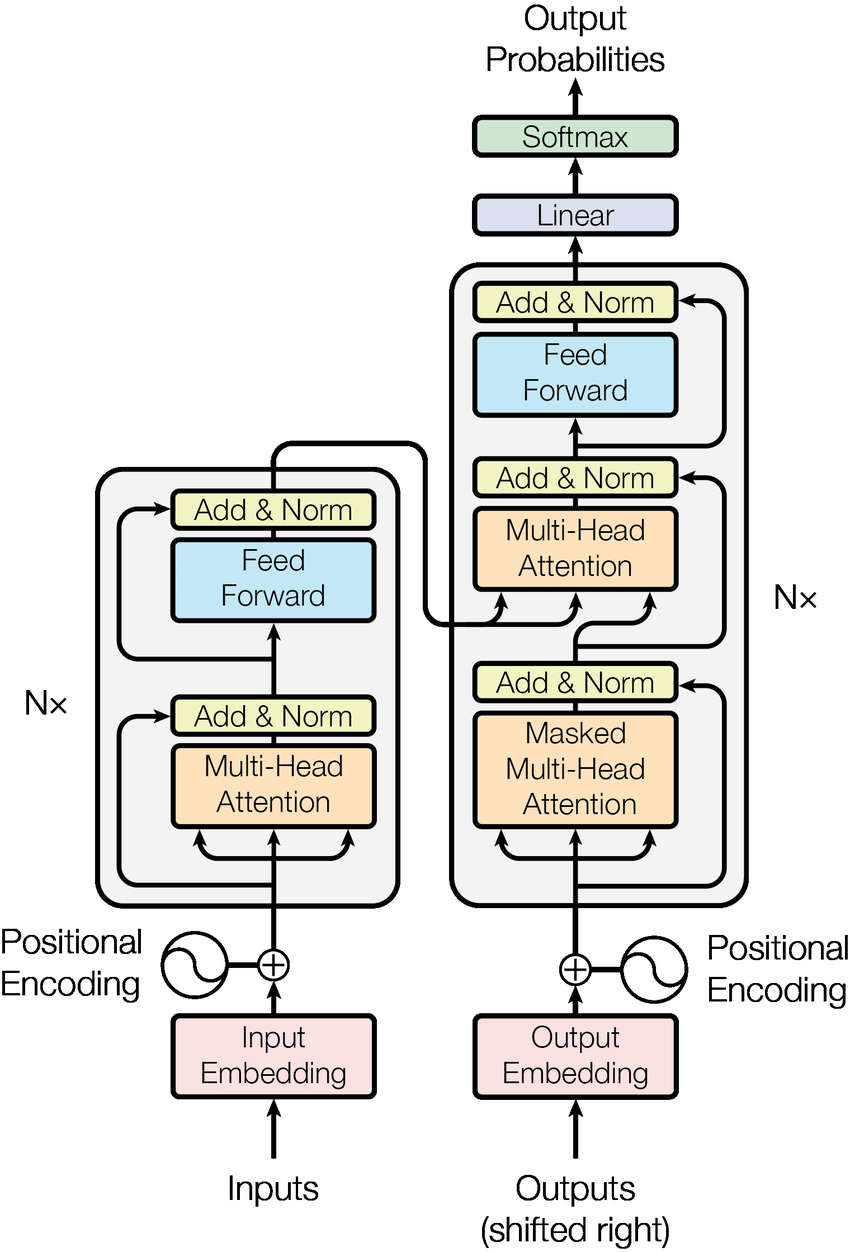
\includegraphics[width=10cm]{figs/chapter2/transformer.png}
    \centering
    \caption{The Transformer architecture. From \citet{vaswani_attention_2023}}
\end{figure}


\subsubsection{Pre-training}

\citet{hadi_LLM_2023}

Learning the patterns and relationships among the data starts with the pre-training process. First, the {\llm} needs to access a vast volume of textual data from multiple sources. The goal of this phase is to predict the succeeding word in a sentence based on the context given by the previous words through unsupervised learning. 

Preparing and preprocessing the data before the training stage is necessary to achieve this. First, demand quality filtering from the training corpus. It is vital to remove unwanted, repetitive, superfluous, and potentially harmful content from the massive text data. Then, according to \citet{hadi_LLM_2023}, duplicate data in a corpus make less diversity of {\llm}. So, the duplication of data will make the training process unstable, impacting the overall performance of the model. Next, it is necessary to pay attention to privacy. The data could have sensitive or personal information, so it is vital to address privacy concerns by removing this information from the pre-training corpus.

An important step, the tokenization, follows this. This step aims to divide the unprocessed text into sequences of individual tokens, which are subsequently input into {\llm}. Moreover, it is vital in mitigating the computational load and enhancing efficiency during the pre-training phase.

\begin{figure}[ht]
    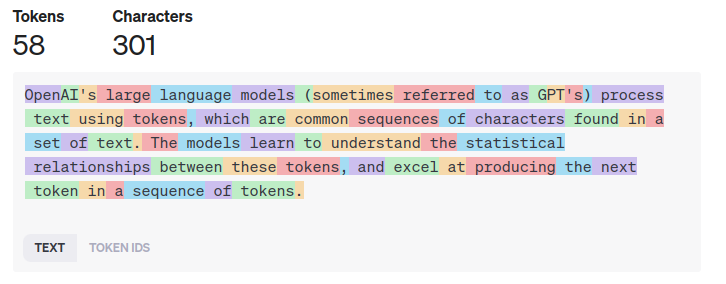
\includegraphics[width=14cm]{figs/chapter2/tokenization.png}
    \centering
    \caption{Tokenization process visually explained by OpenAI \cite{noauthor_openai_nodate}}
\end{figure}

After the pre-training process, the {\llm} goes through a fine-tuning phase.


\subsubsection{Fine-tuning}

\citet{hadi_LLM_2023}

During pre-training, models are generally trained with the objective of next token prediction, learning the nuances of language structure and semantics. According to [Generative pre-trained transformers (GPT) for surface engineering] and \citet{hadi_LLM_2023}, the fine-tuning phase involves adapting a pre-trained model to specific tasks and aligning it with human preferences, improving the performance on particular domains.

In this stage, the model is presented with labeled data to produce more contextually accurate responses for the specific task. Fine-tuning enables the {\llm} to specialize in diverse applications, ranging from language translation and question-answering to text generation. 

Some approaches could be applied to fine-tune the model. \citet{naveed_comprehensive_2023} distinguishes some of them, such as Parameter-Efficient Tuning. As {\llm} typically requires a lot of computational resources, like memory and computing, this approach is helpful because it allows the model to train by updating fewer parameters, adding new ones, or selecting existing ones. Inside this approach, there are also some different methods. The commonly used indicated by \citet{naveed_comprehensive_2023} are Prompt Tuning, Prefix Tuning, and Adapter Tuning.

The Prompt Tuning method integrates trainable prompt token embeddings as prefixes or freely within input token embeddings. During fine-tuning, only the parameters associated with these embeddings are updated for the specific task. At the same time, the remaining model weights remain frozen, facilitating task adaptation without compromising pre-existing knowledge.

In Prefix Tuning, task-specific trainable prefix vectors are introduced to transformer layers, with only the prefix parameters undergoing fine-tuning, while the remaining model parameters remain unchanged. These added prefixes function as virtual tokens, allowing input sequence tokens to attend to them during processing.

Meanwhile, in adapter tuning, an encoder-decoder module is incorporated with the attention and feed-forward layers within the transformer block. The fine-tuning process selectively targets these layers, leaving the remainder of the model frozen to preserve existing knowledge.


% \subsubsection{Parameters}

% The parameters in neural networks function as learnable components that include weights and biases. These values are adjusted during the training process to minimize the difference between the model's predictions and the actual target outputs.

% The more parameters {\llm} have, the more flexibility it has in capturing patterns and relationships in data, but the risk of overfitting increases, and it needs more computational power.

% So ....


\subsection{Comparation between LLM}

The best way to compare {\llm} is to evaluate the model's performance, conforming to \citet{hadi_LLM_2023}. \citet{hadi_LLM_2023} identified five factors to make this comparison: the size of the training corpus, the quality of the training corpus, the number of parameters, the complexity of the model, and some test tasks.


%% FAZER MAIS TARDE E PERGUNTAR AO TIAGO


\subsection{Limitations}

It is safe to say that {\llm} are significantly impacting the world. According to \citet{liu_prompting_nodate}, this is justified by their abilities, mainly in-context learning, reasoning for complex content, instruction following, and creative capacity.

However, {\llm} has some limitations. \citet{hadi_LLM_2023} address some of them, and the most important ones are biased responses, hallucination, explainability, and cyber-attacks. 

We already know that {\llm} are pre-trained with extensive training data. But suppose that data contains some biased information related to factors such as gender, socioeconomic status, and/or race. In that case, this may result in analyses and recommendations that are discriminatory or inaccurate across diverse domains. The problem of bias applies not only to training data but also to user interaction bias, algorithmic bias, and contextual bias. The user interaction bias means that, as user prompts shape responses, and if users consistently ask biased or prejudiced questions, the model may acquire and reinforce these biases in its replies.

A severe limitation that is an active area of research is hallucination. \citet{hadi_LLM_2023} characterized {\llm} hallucinations as when the model attempts to fill gaps in knowledge or context, relying on learned patterns during training. Such occurrences can result in inaccurate or misleading responses, detrimental to the user and the model's reliability.

The way the {\llm} makes decisions is unknown. Comprehending the decision-making process of a complex model with billions of parameters, like {\llm}, is challenging. So, the explainability of these models is a big limitation. Sometimes, it is necessary to decipher the factors that influenced an {\llm}'s decision, and this limitation poses difficulties in offering a clear and concise explanation. In vital sectors like healthcare, where decisions carry substantial consequences, ensuring transparency and the capability to elucidate the model's predictions is essential.

Another limitation is the cyber-attacks. A {\llm} can suffer some prompt injections from a malicious user to extract sensitive information from the model. This is called the Jail Break attack. Another attack is Data Poisoning Attacks, which consist in data poisoning strategies to manipulate the model's output.

Furthermore, \citet{liu_prompting_nodate} highlighted another limitation: the temporal lag of the training corpus. {\llm} cannot retrieve information in real time, and the answer generated may not be the most current.

It is important to be aware of these limitations.


\section{Conversational Virtual Assistant}

Conversational Agents, also known as chatbots, chatterbots, or virtual assistants, have become a vital aspect of the digital landscape. These tools are generally dialogue systems that understand, interpret, and generate human language, enabling them to communicate with users to dissolve their questions.

Chatbots are increasingly being used in various contexts due to their many benefits. 
These aspects that make companies bet on the use of chatbots are the continuous availability to support and assist the customer, ensuring more consistent support, the cost-efficiency by reducing the human customer support, the time-saving both for the organization and for customers due to the immediate responses to the user queries, the ease and intuitiveness of this systems, improve service with every interaction. Because of this, the utility of the chatbots as tools is increasing as the technology advances. 

The rise of conversational virtual assistants is underpinned by a convergence of technologies, including {\nlp}, {\mlearning}, and {\ai}.

In this section, I explored the implementation of chatbots, their components, and existing tools.


\subsection{Overview of Conversational Virtual Assistants}

\citet{nuruzzaman_survey_2018} separated chatbot applications based on their main features and functionalities. There are four chatbot models: goal-based, knowledge-based, service-based, and response generated-based. Goal-based chatbots are designed for particular tasks and structured to engage in concise conversations to collect user information for task completion.

% escrever mais sobre isto mas tirar as dúvidas: artigo confuso, perguntar ao joão !!!!

\citet{borah_survey_2019} said that the process of response generation is not the same for all chatbots and distinguished them into four models: Retrieval-Based, Generative-Based, Long and Short Conversation, and Open or Close Domain. \citet{chizhik_challenges_2020} are in line with \citet{borah_survey_2019}, and divided chatbots into three categories based on response generation architectures: rule-based chatbots, retrieval-based chatbots, and generative-based chatbots.

According to \citet{chizhik_challenges_2020}, a rule-based chatbot examines fundamental features of the user's input statement and generates a response based on a predetermined set of manually crafted templates.

Conforming to \citet{chizhik_challenges_2020} and \citet{borah_survey_2019}, a retrieval-based chatbot picks a response from an extensive precompiled dataset. It selects the most promising reply from the top-k ranked candidates. Thus, they refrain from producing new text. It has limited flexibility regarding domain since they are usually applied to one domain, and in terms of errors, because, for example, the user cannot make grammatical mistakes.

A generative-based chatbot generates a text sequence as a response rather than choosing it from a predefined set of candidates. These chatbots are very flexible and can handle open domains because they are implemented with Machine Translation techniques. The interactions will be more identical to those of humans, as it implements a self-learning method from a large quantity of interaction data. However, this could be complex and costly to implement.

Beyond that, \citet{borah_survey_2019} compare long and short conversations. He concluded that a more extended conversation requires saving what has been said, which makes it challenging to automate, unlike a short conversation. 

Also, \citet{borah_survey_2019} defined the differences between chatbots with opened or closed domains. In an open-domain environment, conversations can go in any direction without a predefined goal or intention. Crafting meaningful responses in such contexts demands an extensive breadth of world knowledge spanning countless topics. Conversely, closed-domain systems have more constrained inputs and outputs, focusing on specific goals. Consequently, many chatbots are inherently closed-domain, designed with a clear objective.


\subsection{Common System Architectures}

Most chatbot implementations apply standard components, such as {\nlp}, dialogue, knowledge, and data storage modules.
According to \citet{ngai_intelligent_2021} and to \citet{dilmegani_cem_how_nodate}, the function of each module can be summarized as follows.

The dialogue module is in charge of handling the conversation flow. To effectively communicate with the user, conversation agents must understand the human language using a {\nlp} Engine to decide what to do with the intention found. 

\begin{figure}[ht]
    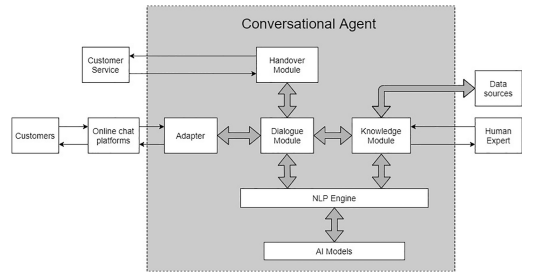
\includegraphics[width=14cm]{figs/chapter2/chatbot_architecture.png}
    \centering
    \caption{[REFAZER IMAGEM] Overview of a conversational system architecture From [An intelligent knowledge-based chatbot for customer service]}
\end{figure}

The knowledge module is the source of data and knowledge of the chatbot. After knowing the user's intention, this module will retrieve the data to respond to the user.

Many chatbots use a knowledge base for the knowledge module. In compliance with \citet{pereira_querying_2023}, this choice is justified because it is advantageous to have the data organized semantically. This establishes a coherent structure for structured and unstructured data, simplifying the deduction of new knowledge.

Additionally, some chatbots are integrated with web scrapers to pull data from online resources and display it to users

% falar das partes da arquitetura, e como essas componentes estão interligadas

\subsection{Generative-Based Chatbot}

Generative-based conversational virtual assistants are chatbots that use generative models to generate natural language responses. These chatbots utilize sophisticated deep-learning techniques, such as {\llm} as a {\nlp} engine to understand the user query and formulate a response in context. The {\llm} has been widely used in the new chatbots.

% \begin{figure}[ht]
%    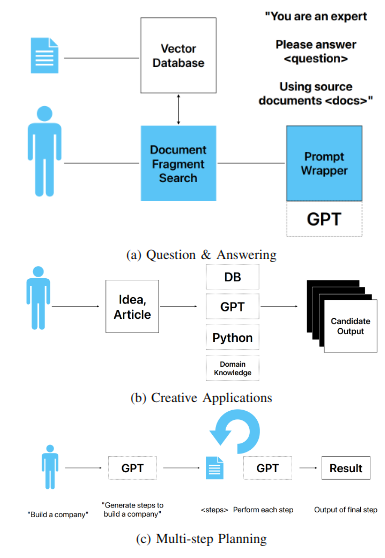
\includegraphics[width=10cm]{figs/chapter2/llm.png}
%    \centering
%    \caption{[REFAZER IMAGEM] Templates for LLM-based application development. GPT is taken as an example scenario representing LLMs From \citet{hadi_LLM_2023}}
% \end{figure}

There are some methods to improve the results of a {\llm} used on chatbot: fine-tuning the {\llm}, {\rag}, and Prompt Engineering.

\begin{figure}[ht]
    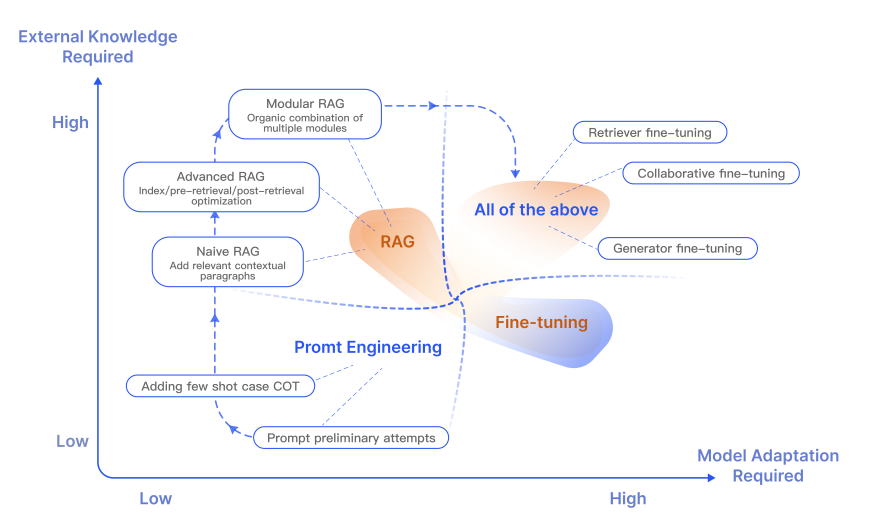
\includegraphics[width=10cm]{figs/chapter2/otimization_generative_chatbot.png}
    \centering
    \caption{[REFAZER IMAGEM] optimization methods of generative-based chatbots. Adapted from [Retrieval-Augmented Generation for Large Language Models: A Survey]}
\end{figure}

The figure above shows how these methods influence model adaptation and external knowledge. Mixing all methods requires a high model adaptation and external knowledge, but provides better results. 

The following sections demonstrate how Prompt Engineering and {\rag} can optimize {\llm}.



\subsection{Prompt Engineering}

With the emergence of new technologies, such as {\llm}, other research fields were born. Prompt Engineering is one of these cases and has been widely applied. In compliance with \citet{mesko_prompt_2023}, this emerging field involves designing, refining, and implementing prompts or instructions to direct the output of {\llm}, aiding in diverse tasks. {\llm} can follow specific directions provided by users in natural language after being tuned with instructions,

\citet{ma_beyond_2023} noted that research demonstrates that thoughtful prompts enhance {\llm} performance across reasoning and planning tasks. This improvement is achieved through intermediate representations involving thoughts, decomposition, search-decomposition mix, structure, abstraction, and optimization.

Also, \citet{ma_beyond_2023} find with their work that prompt engineering has many benefits for the user when it is well implemented because prompt-based methods assist humans in forming mental models for problem-solving. Also, they conclude that task decomposition enables the breakdown of a complex task into specific sub-tasks, each matched with readily available tools suitable for its completion. This method of prompting engineering had very successful results.

\begin{figure}[ht]
    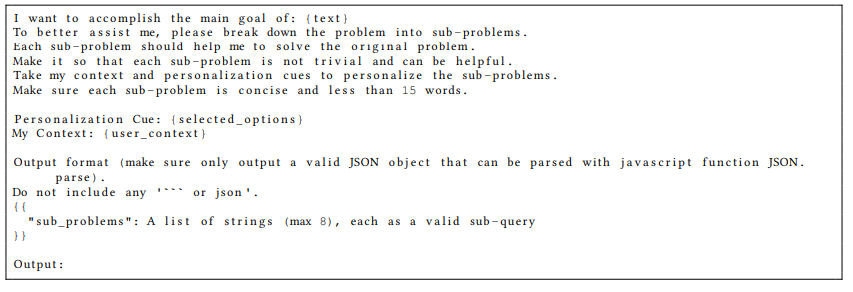
\includegraphics[width=14cm]{figs/chapter2/prompt.png}
    \centering
    \caption{[REFAZER IMAGEM] Example of a prompt that applies task decomposition From \citet{ma_beyond_2023}}
\end{figure}


\citet{mesko_prompt_2023} raise a series of recommendations for more effective {\llm} prompts: it must be as precise as possible; providing the setting and the context of the question is essential; describe the goal of the prompt first; give a role to the {\llm} to get more context (for example, "You are a math teacher and explain the natural numbers"); continuous {\llm} prompt refinement; prefer open questions over close-questions. Regularly testing prompts in real-world situations is crucial, as their effectiveness is most accurately assessed through practical application.


\subsection{Retrieval-Augmented Generation (RAG)}

\citet{gao_retrieval-augmented_2023} made a survey into {\rag} systems and distiguish the parametric knowledge from non-parametric knowledge. Traditionally, {\llm} can adapt their knowledge and responses to a specific domain by fine-tuning models with parameters. This is \textbf{parametric knowledge} because the {\llm} knowledge is provided through the model's training data. However, entirely parameterized {\llm} have limitations, including challenges in retaining all the knowledge during training, the inability to dynamically update model parameters, leading to outdatedness, and hallucination. The \textbf{non-parametric knowledge}, provided by external information sources, emerged to solve these limitations.

This non-parametric knowledge approach is known as {\rag}. So, according to \citet{gao_retrieval-augmented_2023}, {\rag} involves retrieving pertinent information from external knowledge bases, giving more context to the {\llm}. This approach was introduced by \citet{lewis_retrieval-augmented_2020} in 2020 and enabled {\llm} to access and utilize up-to-date or domain-specific information to enhance response accuracy and relevance while reducing hallucinations.


\subsubsection{Workflow of a {\rag} system}

The following figure shows the workflow of a {\rag}. This model aims to retrieve pertinent information from an extensive corpus of documents when answering questions or generating text, subsequently utilizing this information to enhance the quality of predictions in compliance with \citet{lewis_retrieval-augmented_2020}.

\begin{figure}[ht]
    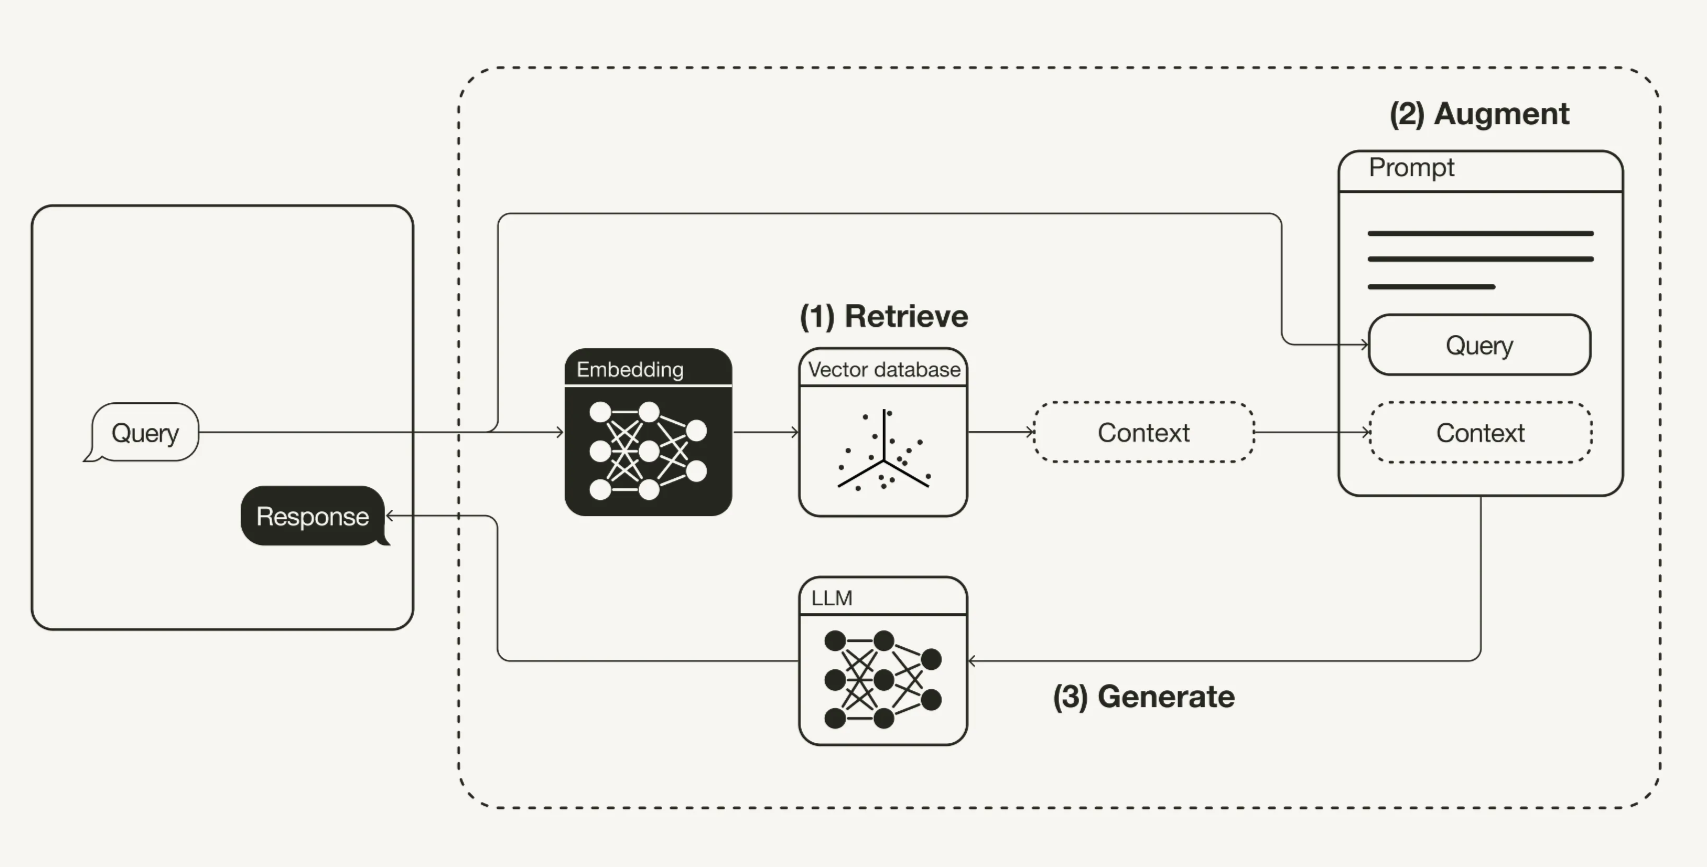
\includegraphics[width=10cm]{figs/chapter2/rag_workflow.png}
    \centering
    \caption{[REFAZER IMAGEM] {\rag} workflow. Adapted from [https://towardsdatascience.com/retrieval-augmented-generation-rag-from-theory-to-langchain-implementation-4e9bd5f6a4f2]}
\end{figure}

\citet{gao_retrieval-augmented_2023} explain in a simple way the workflow. The first step is 1) Retrieve information from an external data source, such as a vector database, as in the example of the figure. According to \citet{gao_retrieval-augmented_2023}, this step utilizes Encoding Models, such as {\bm}, to retrieve relevant information based on the query. The second step is 2) Augment, improving the {\llm} prompt with the context retrieved from external data sources. The last step is 3) Generation. Using the prompt with the retrieved context, the {\llm} generates a response to the query.


% escrever mais? vantagens,  RAG vs Fine-tuning, tipos de RAG


\section{Interactive Query Builder}

A query builder refers to constructing a query according to the user preferences. This query could be in different formats, such as SQL [Domain Specific Query Generation from Natural Language Text] and RDF [A Front-End Approach for User Query Generation and Information Retrieval in the SemanticLIFE Framework]. 

It is important to note that there aren't many cases of query builder documentation.



\section{Insights/Summary}

Não há muito trabalho feito para o desenvolvimento de Conversational Queries Builder.

>> limitations: 

* não existe query builder para dados médicos

* muitos chatbots com o seguinte flow: NLP -> query struct -> DB, que não é o caso a ser implementado

* há algumas limitações dos chatbots a ter em conta, destaco os erros gramaticais, erros ortográficos e a ambiguidade de textos

* Recommender System: Existing chatbots do not ask questions, explain, or advise the user topic. They collect information and provide responses from the knowledge base. The chatbot should be able to write questions based on previous answers. [referencia: Chatbot Implementation in Customer Service Industry through Deep Neural Networks]

* alucianação dos LLM

>> oportunidades:

* a união entre as áreas de NLP e de IR pode mostrar-se muito promissora

* vários modelos de AI em NLP sobre várias sub-áreas: Query understanding, Text Classification e Text Generation
\chapter{Methodology}
\label{chapter:Methodology}

For this thesis work, after an extensive literature review on crucial fields, concepts and technologies, we are ready to achieve the primary goal of this work.

This section presents the methodology applied to this project, from the work done to the work plan.

\section{Work Done}

This semester's work was mainly focused on state-of-the-art understanding and writing, going through a process of research and reading articles. The state-of-the-art objectives established in \autoref{chapter:Introduction} have been completed. These objectives are to study methodologies to build a conversational user interface, procedures to retrieve the databases of most interest and explore the definition of a study protocol. It was essential not only to learn more about the actual state of some technologies and concepts but also to get more into the project goal and requirements.

In terms of development, first, I built a prototype of an architecture, which is shown in figure \ref{fig_arch}, and then started the development.

\begin{figure}[ht]
    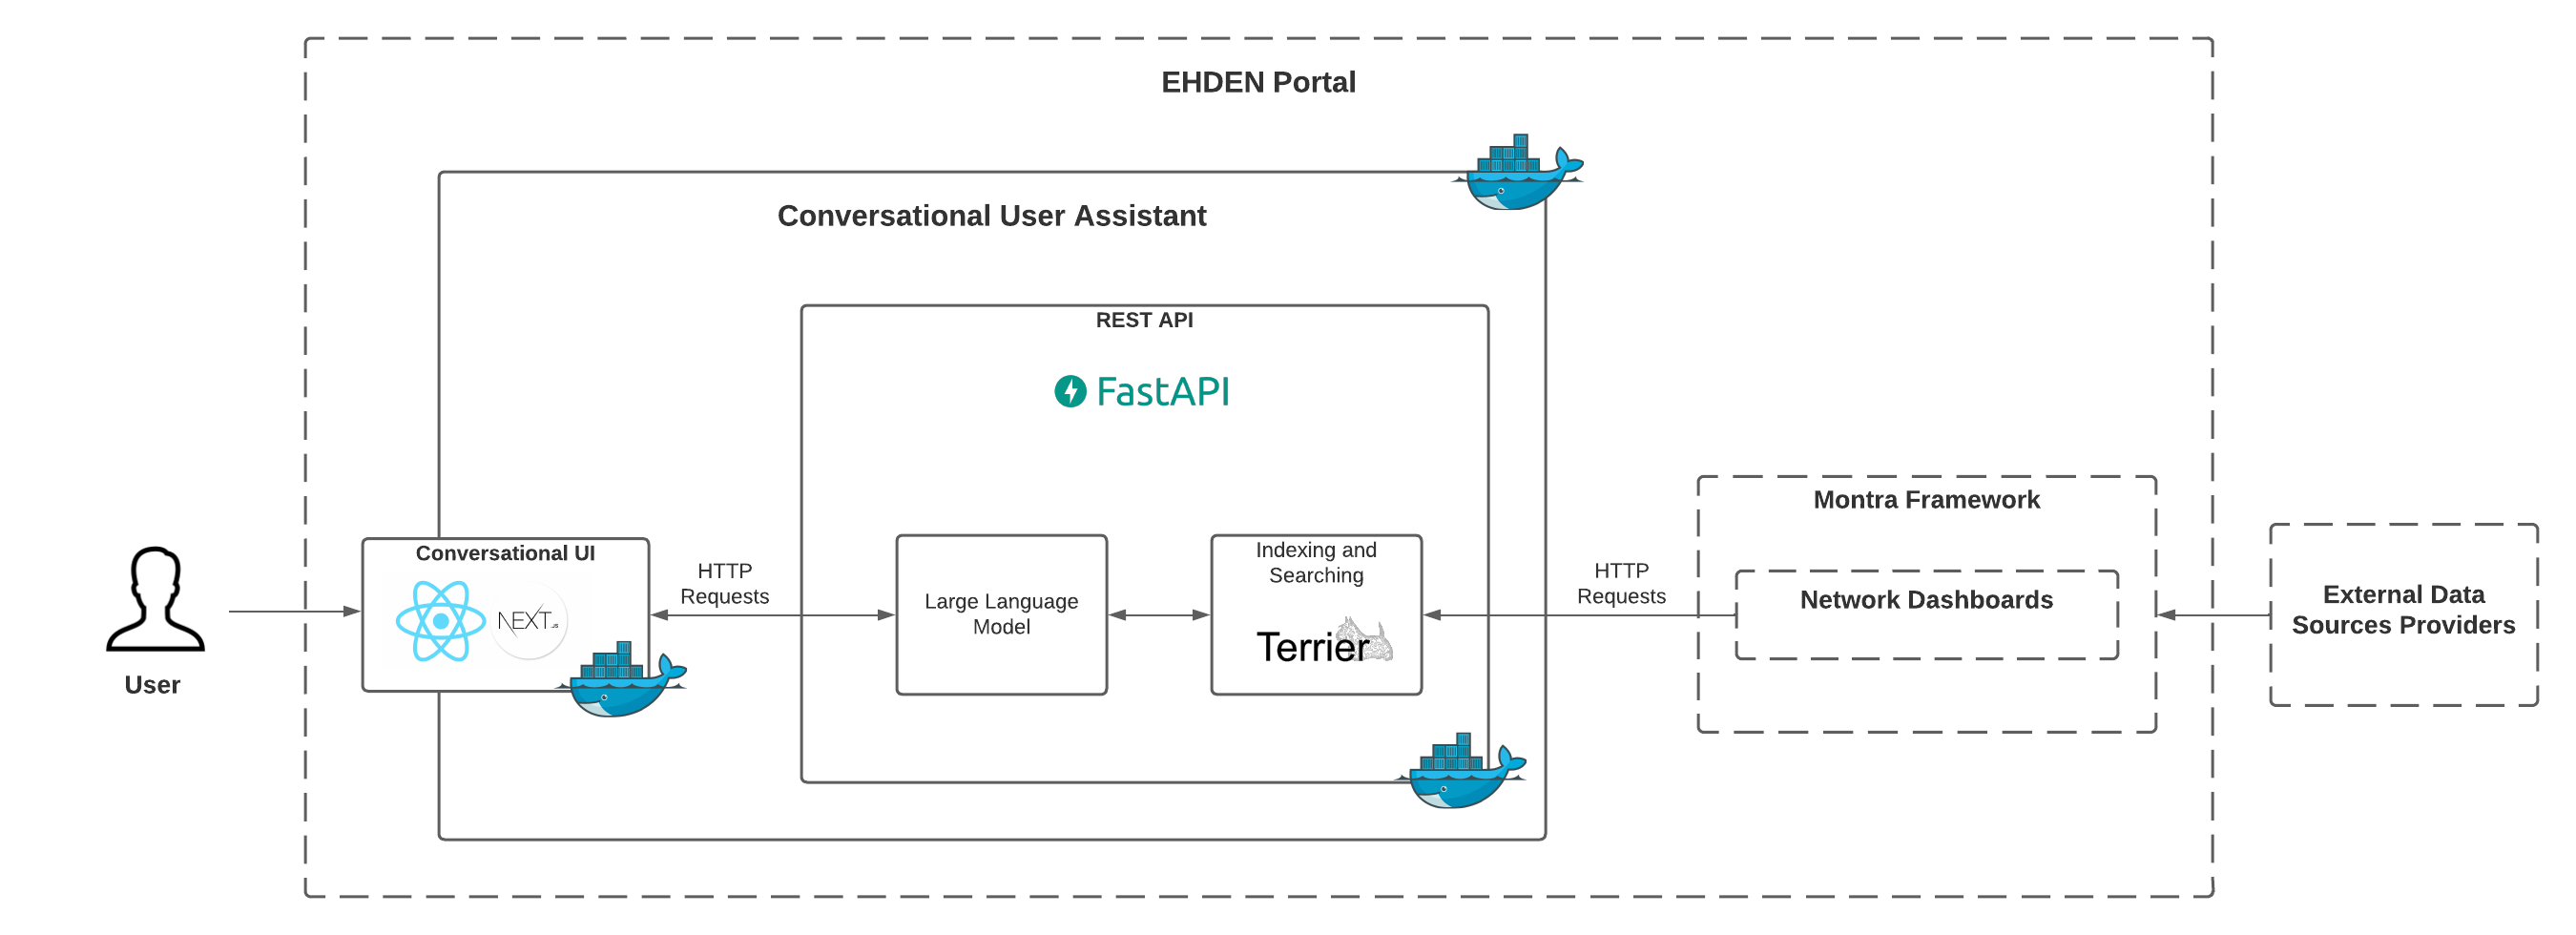
\includegraphics[width=16cm]{figs/chapter3/arquitetura.png}
    \centering
    \caption{Architecture Proposal. Only the components with a solid line relate to the proposed work.}
    \label{fig_arch}
\end{figure}

I have developed a prototype of a chat-like interface using NextJS, a well-known ReactJS framework. Also, I have developed a REST API in FastAPI, a modern web framework based on Python. The interface and the API communicate between them through HTTP requests. The components of this application are deployed in Docker containers.

Beyond this, inside the backend module, I have started implementing and testing a {\bm} method to retrieve the best databases for a given user query. First, {\nlp} methods are applied to understand the plain-text query. For now, the {\nlp} method is in a very simple stage, because only tokenization, normalization, stemming and lemmatization are applied. Then, the {\bm} score is calculated between the query and the concepts of which database, making a database ranking. To implement the {\ir} technique, I am using the pyterrier library, and it could be changed to another library later if I discover another one more effective. The PyTerrier library facilitates the creation of a collection, allowing for the indexing and searching of data using a {\bm} method.
 
So, for now, the application developed can receive a user query through the frontend module and then, the backend module retrieves a rank of databases based on the query understanding. The chatbot interaction with the user is limited, as shown in figure \ref{fig_interface}. When the chatbot identifies a concept, he retrieves a list of clickable buttons of the ranked databases, indicating the database ID and its {\bm25} score. However, if it doesn't, it sends a pre-defined message.

\begin{figure}[ht]
    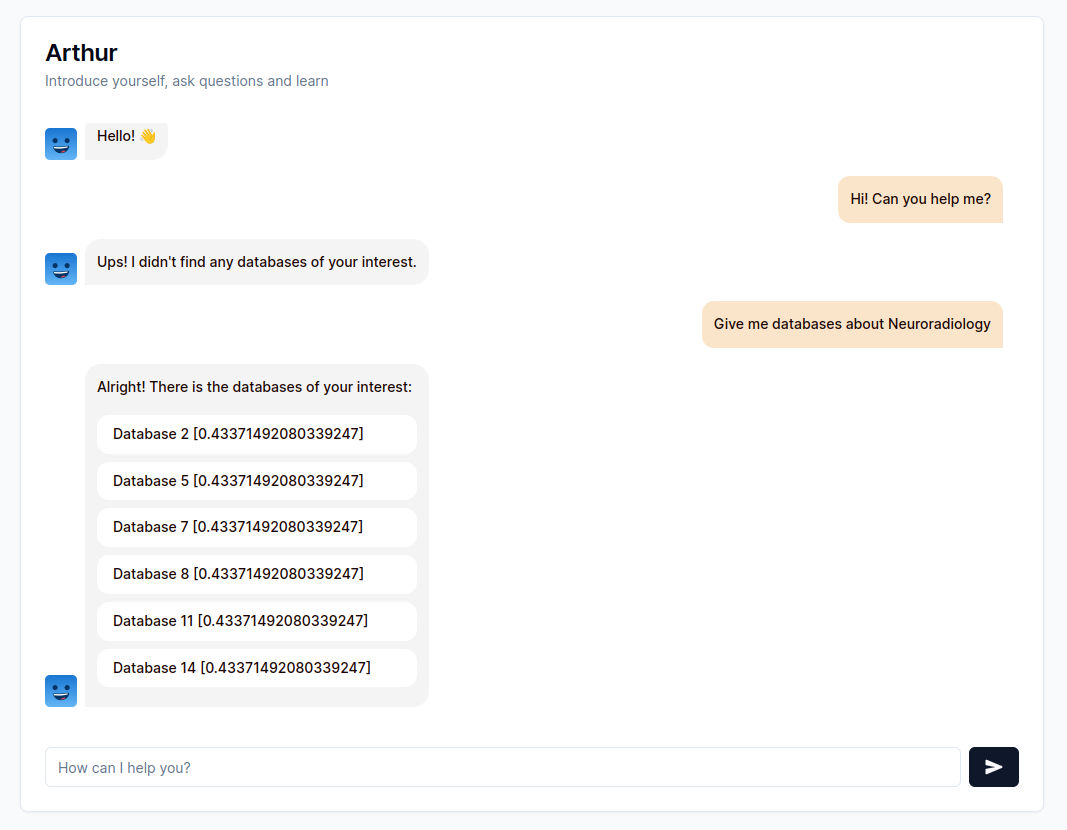
\includegraphics[width=12cm]{figs/chapter3/interface.png}
    \centering
    \caption{Example of an interaction with the chatbot, showing the current state of the project.}
    \label{fig_interface}
\end{figure}



\section{Future work}

For the following months, I will continue the development of the database recommendation, based on {\bm}, improving some aspects, like concept linking. Also, test and improve this {\ir} implementation based on the testing results. 

After this, I will choose, implement, and fine-tune a {\llm} in order to guide the conversation to build the final query with the cohort definition structure. By doing this, the conversation flows naturally. Finally, test and improve the model based on the testing results.

The next step is integrating this system in the {\ehden} Portal and testing and validating the system. 

The documentation of the implementation and the respective steps taken will be carried out throughout its development.

The subsection \ref{workplan} presents a plan for all these tasks.


\section{Work Plan}
\label{workplan}

The following Gantt diagram, figure \ref{fig_gantt}, shows the work proposal for the following months. This diagram is divided into two semesters: the first refers to the work done in the first semester, and the second to the work proposed for the second semester.

\begin{figure}[ht]
    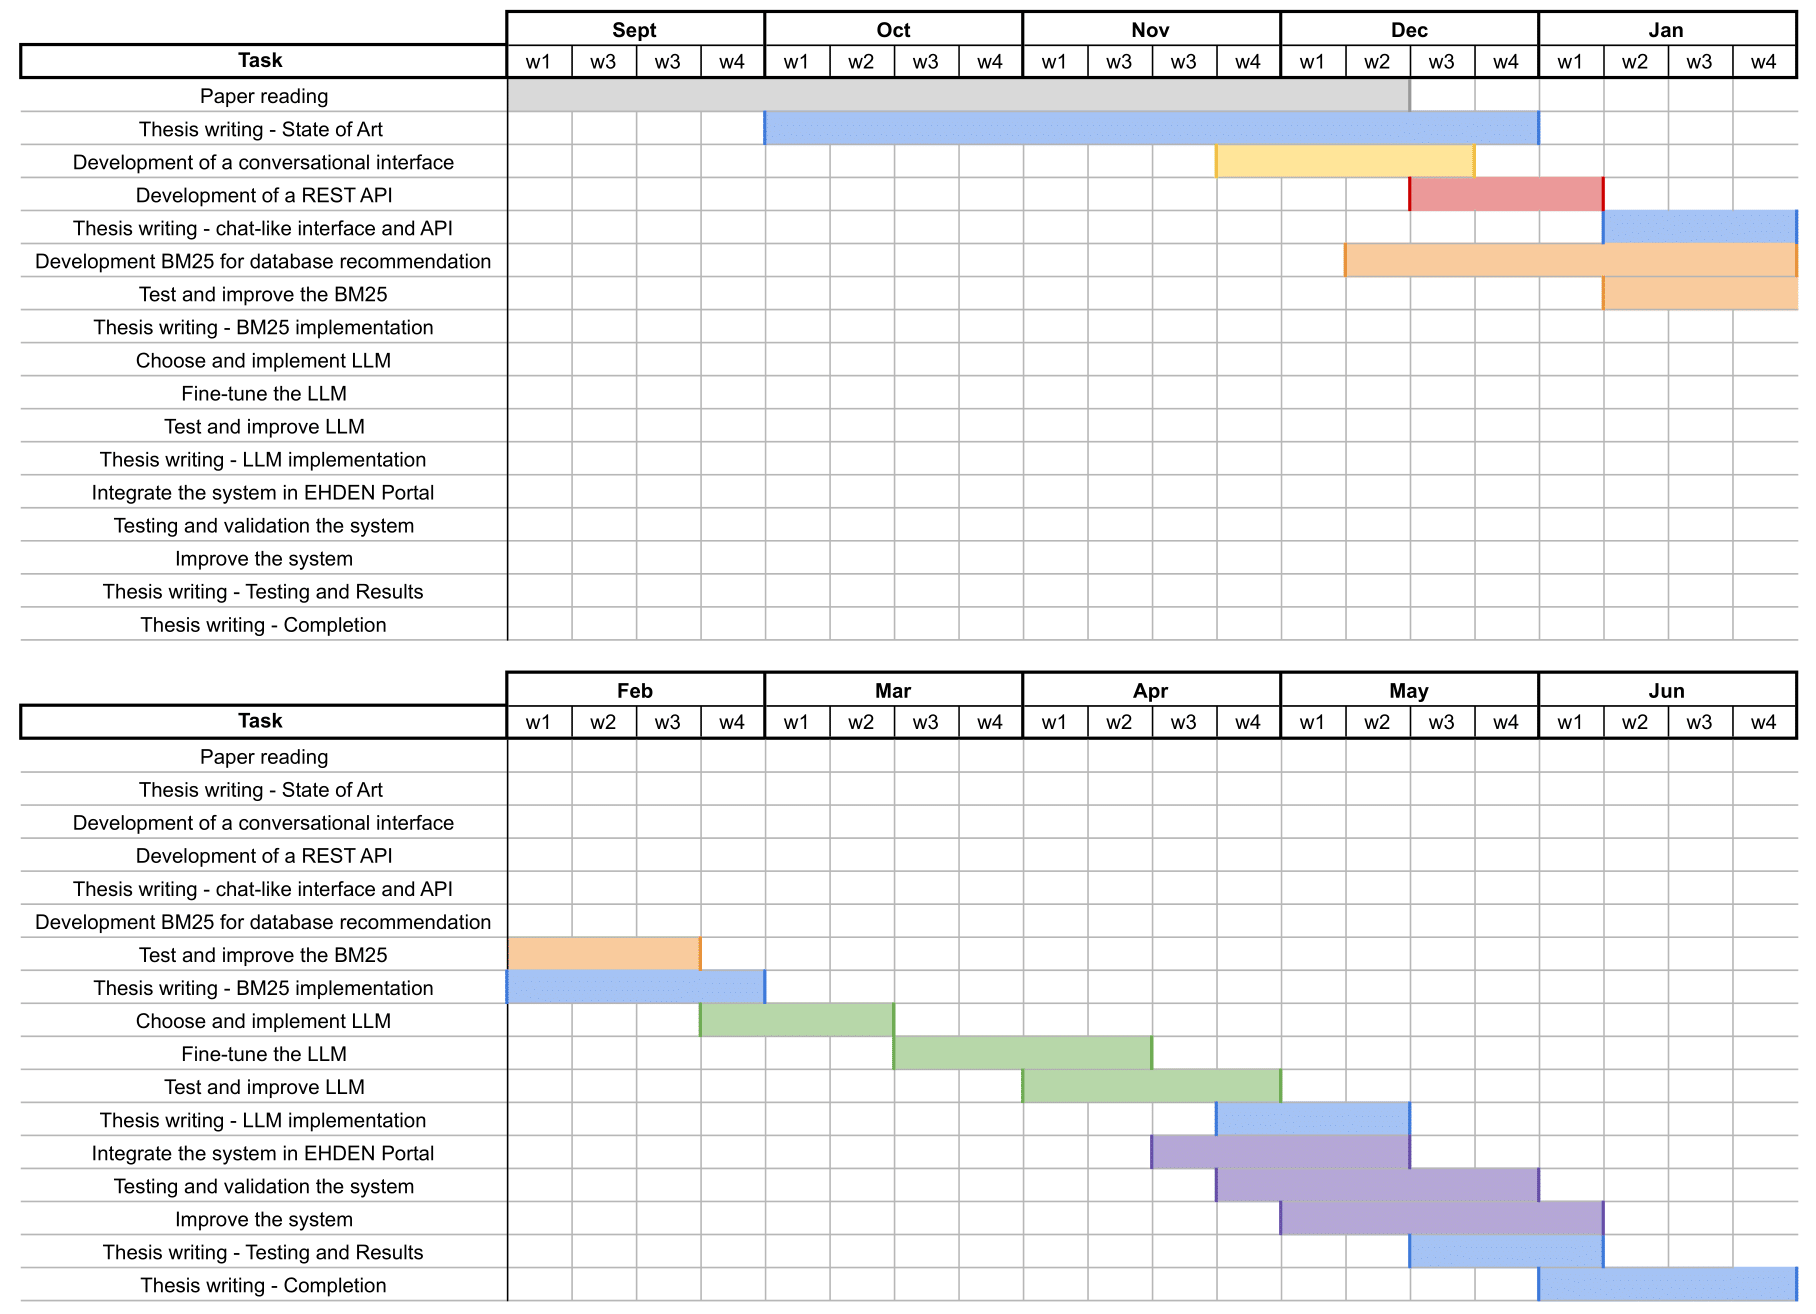
\includegraphics[width=16cm]{figs/chapter3/diagram_gantt.png}
    \centering
    \caption{Proposal thesis work in a Gantt Diagram.}
    \label{fig_gantt}
\end{figure}


%%%%%%%%%%%%%%%%%%%%%%%%%%%%%%%%%%%%%%%%%%%%%%%%%%%%%%%
% End of Thesis text 
%%%%%%%%%%%%%%%%%%%%%%%%%%%%%%%%%%%%%%%%%%%%%%%%%%%%%%%

\backmatter

%%%%%%%%%%%%%%%%%%%%%%%%%%%%%%%%%%%%%%%%%%%%%%%%%%%%%%%
% Print all used references
%%%%%%%%%%%%%%%%%%%%%%%%%%%%%%%%%%%%%%%%%%%%%%%%%%%%%%%

\begingroup
\renewcommand{\bibfont}{\footnotesize}
% Redefine References name to Portuguese
% Change if you are using English
\defbibheading{bibliography}[References]{
	\chapter{#1}
}
\SingleSpacing
\setlength\bibitemsep{8pt}
\printbibliography[heading=bibliography]
\endgroup


%%%%%%%%%%%%%%%%%%%%%%%%%%%%%%%%%%%%%%%%%%%%%%%%%%%%%%%
% Load appendix
%%%%%%%%%%%%%%%%%%%%%%%%%%%%%%%%%%%%%%%%%%%%%%%%%%%%%%%

\mainmatterWithoutReset
\appendix

% \include{appendix-a}
% \include{appendix-b}
% \include{appendix-c}

\end{document}
